\documentclass[11pt]{article}
\usepackage[a4paper,margin=1in]{geometry}
\usepackage[T1]{fontenc}
\usepackage[utf8]{inputenc}
\usepackage{lmodern}
\usepackage{graphicx}
\usepackage{booktabs}
\usepackage{array}
\usepackage{tabularx}
\usepackage{longtable}
\usepackage{hyperref}
\usepackage{xcolor}
\usepackage{float}
\usepackage{caption}
\usepackage{subcaption}
\usepackage{enumitem}
\usepackage{tikz}
\usetikzlibrary{arrows.meta,positioning,shapes.geometric,fit}

\hypersetup{
    colorlinks=true,
    linkcolor=blue,
    urlcolor=blue
}

\definecolor{gptblue}{HTML}{0F6CBD}
\definecolor{llavagreen}{HTML}{2F7D32}
\definecolor{qwenorange}{HTML}{C76B00}
\definecolor{softgray}{HTML}{F2F4F7}

\title{A Human Comparison of GPT-4.1, LLaVA-7B, and Qwen2.5-VL}
\author{}
\date{May 8, 2026}

\newcommand{\modelbox}[3]{
    \node[
        draw=#1!80!black,
        fill=#1!10,
        rounded corners,
        minimum width=3.0cm,
        minimum height=0.95cm,
        align=center
    ] (#2) {#3};
}

\begin{document}
\maketitle

\section{What This Report Is Actually Comparing}
This report compares the three strongest models in the current repository benchmark sweep:
\texttt{gpt-4.1}, \texttt{llava-7b}, and \texttt{qwen25-vl}. The quantitative results come directly from the regenerated comparison outputs in \texttt{comparison/output/}. In the local codebase, \texttt{qwen25-vl} maps to \texttt{Qwen/Qwen2.5-VL-3B-Instruct}, while \texttt{llava-7b} maps to \texttt{llava-hf/llava-1.5-7b-hf}. The OpenAI wrapper in \texttt{models/gpt4.py} currently defaults to \texttt{gpt-4o}, but the saved benchmark files and the regenerated comparison report include a separate \texttt{gpt-4.1} result set, so this document follows the comparison outputs rather than the wrapper default.

The benchmark suite covers 21 saved tasks across four families:
captioning, question answering, labeling, and detection. The comparison report was rebuilt locally on May 8, 2026 using:

\begin{verbatim}
$env:PYTHONPATH='.'; python comparison\build_report.py
\end{verbatim}

\section{Short Version}
If you only want the conclusion, it is this:
\begin{itemize}[leftmargin=*]
    \item \texttt{gpt-4.1} is the best all-around model in this run if you care most about average score and labeling-heavy tasks.
    \item \texttt{qwen25-vl} is the most consistently competitive model, wins the most individual benchmarks, and is especially strong on captioning.
    \item \texttt{llava-7b} is the best open-weight baseline here in the sense that it stays surprisingly close to the leaders on many tasks, but it is not quite as broad or as robust.
\end{itemize}

That is the simple story. The more interesting story is \emph{why} they separate the way they do.

\section{Headline Numbers}
\begin{table}[H]
\centering
\caption{Overall comparison numbers from \texttt{comparison/output/model\_summary.csv}.}
\begin{tabular}{>{\ttfamily}lrrrr}
\toprule
Model & Mean score & Normalized & Mean rank & 1st places \\
\midrule
gpt-4.1 & 0.518 & 0.758 & 2.10 & 10 \\
qwen25-vl & 0.478 & 0.727 & 1.95 & 11 \\
llava-7b & 0.467 & 0.661 & 2.14 & 7 \\
\bottomrule
\end{tabular}
\end{table}

\noindent
These three models are closer than a casual glance suggests. \texttt{gpt-4.1} has the best average score, but \texttt{qwen25-vl} has the best average rank and the most first-place finishes. That means \texttt{gpt-4.1} is slightly better \emph{on average}, while \texttt{qwen25-vl} is more often at or near the top of a given benchmark. \texttt{llava-7b} is a small step behind both, but not by enough to treat it as a different class of model.

\begin{table}[H]
\centering
\caption{Family-level performance from \texttt{comparison/output/family\_summary.csv}.}
\begin{tabular}{>{\ttfamily}l>{\ttfamily}lrrr}
\toprule
Model & Family & Mean score & Mean rank & Mean normalized \\
\midrule
qwen25-vl & captioning & 0.325 & 1.50 & 0.977 \\
llava-7b & captioning & 0.325 & 1.75 & 0.936 \\
gpt-4.1 & captioning & 0.260 & 3.50 & 0.715 \\
\midrule
qwen25-vl & qa & 0.533 & 2.00 & 0.726 \\
llava-7b & qa & 0.367 & 3.33 & 0.433 \\
gpt-4.1 & qa & 0.400 & 3.67 & 0.333 \\
\midrule
gpt-4.1 & labeling & 0.764 & 1.36 & 0.877 \\
llava-7b & labeling & 0.673 & 1.82 & 0.712 \\
qwen25-vl & labeling & 0.618 & 2.27 & 0.627 \\
\midrule
gpt-4.1 & detection & 0.080 & 1.33 & 0.806 \\
qwen25-vl & detection & 0.111 & 1.33 & 0.765 \\
llava-7b & detection & 0.000 & 2.67 & 0.333 \\
\bottomrule
\end{tabular}
\end{table}

\section{How The Three Models Work Internally}
\subsection{GPT-4.1}
OpenAI does not publish a full layer-by-layer architecture for \texttt{gpt-4.1}, so the diagram below is the public-facing view rather than a reverse-engineered claim. What is public is that \texttt{gpt-4.1} accepts image input, uses a very long context window, and is optimized for strong instruction following and tool use.\footnote{\url{https://developers.openai.com/api/docs/models/gpt-4.1}} The local wrapper in \texttt{models/gpt4.py} sends an image and prompt to the Responses API as a multimodal user message.

\begin{figure}[H]
\centering
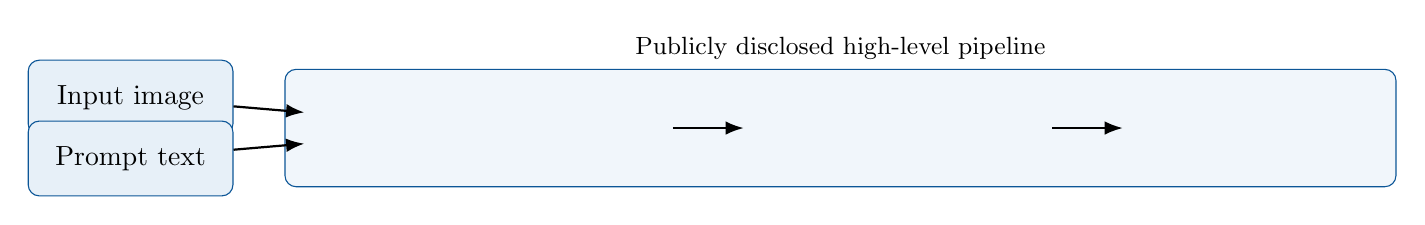
\begin{tikzpicture}[node distance=1.4cm and 0.9cm,>=Latex]
    \modelbox{gptblue}{gptenc}{Vision encoder\\and multimodal tokenization}
    \node[left=of gptenc, yshift=11pt, draw=gptblue!80!black, fill=gptblue!10, rounded corners, minimum width=2.6cm, minimum height=0.95cm, align=center] (gptimg) {Input image};
    \node[left=of gptenc, yshift=-11pt, draw=gptblue!80!black, fill=gptblue!10, rounded corners, minimum width=2.6cm, minimum height=0.95cm, align=center] (gpttext) {Prompt text};
    \node[right=of gptenc, draw=gptblue!80!black, fill=gptblue!10, rounded corners, minimum width=3.2cm, minimum height=0.95cm, align=center] (gptcore) {Proprietary GPT-4.1\\multimodal transformer};
    \node[right=of gptcore, draw=gptblue!80!black, fill=gptblue!10, rounded corners, minimum width=3.0cm, minimum height=0.95cm, align=center] (gpthead) {Autoregressive text\\decoder/output};

    \node[draw=gptblue!80!black,fill=gptblue!6,rounded corners,fit=(gptenc)(gptcore)(gpthead),inner sep=7pt,label=above:{\small Publicly disclosed high-level pipeline}] {};

    \draw[->,thick] (gptimg) -- (gptenc);
    \draw[->,thick] (gpttext) -- (gptenc);
    \draw[->,thick] (gptenc) -- (gptcore);
    \draw[->,thick] (gptcore) -- (gpthead);
\end{tikzpicture}
\caption{High-level view of the \texttt{gpt-4.1} inference path used in this repo.}
\end{figure}

\subsection{LLaVA-7B}
LLaVA-1.5-7B is much more transparent. Its standard recipe is a CLIP-style vision encoder, a learned projector that maps image features into the language model token space, and a Vicuna/LLaMA-family decoder-style transformer fine-tuned on visual instruction data.\footnote{\url{https://huggingface.co/llava-hf/llava-1.5-7b-hf}} In this repo, the wrapper loads \texttt{LlavaForConditionalGeneration} plus an \texttt{AutoProcessor}, prepares a chat-style prompt, and generates text autoregressively.

\begin{figure}[H]
\centering
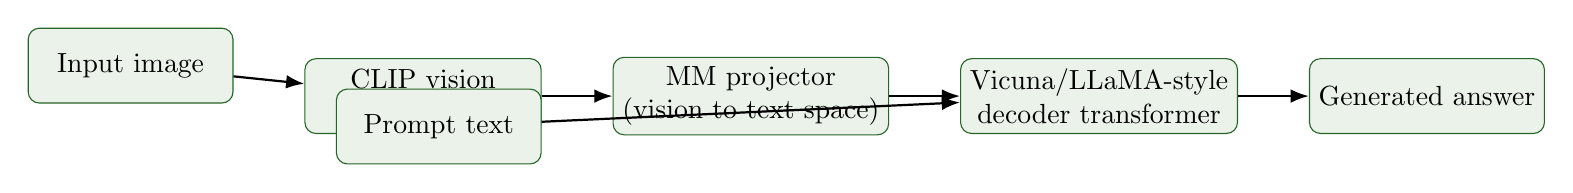
\begin{tikzpicture}[node distance=1.4cm and 0.9cm,>=Latex]
    \modelbox{llavagreen}{llavavit}{CLIP vision\\encoder}
    \node[left=of llavavit, yshift=11pt, draw=llavagreen!80!black, fill=llavagreen!10, rounded corners, minimum width=2.6cm, minimum height=0.95cm, align=center] (llavaimg) {Input image};
    \node[right=of llavavit, draw=llavagreen!80!black, fill=llavagreen!10, rounded corners, minimum width=3.0cm, minimum height=0.95cm, align=center] (llavaproj) {MM projector\\(vision to text space)};
    \node[left=of llavaproj, yshift=-11pt, draw=llavagreen!80!black, fill=llavagreen!10, rounded corners, minimum width=2.6cm, minimum height=0.95cm, align=center] (llavatext) {Prompt text};
    \node[right=of llavaproj, draw=llavagreen!80!black, fill=llavagreen!10, rounded corners, minimum width=3.3cm, minimum height=0.95cm, align=center] (llavalm) {Vicuna/LLaMA-style\\decoder transformer};
    \node[right=of llavalm, draw=llavagreen!80!black, fill=llavagreen!10, rounded corners, minimum width=2.6cm, minimum height=0.95cm, align=center] (llavaout) {Generated answer};

    \draw[->,thick] (llavaimg) -- (llavavit);
    \draw[->,thick] (llavavit) -- (llavaproj);
    \draw[->,thick] (llavaproj) -- (llavalm);
    \draw[->,thick] (llavatext) -- (llavalm);
    \draw[->,thick] (llavalm) -- (llavaout);
\end{tikzpicture}
\caption{Typical LLaVA-1.5-7B architecture, which matches the repo's \texttt{llava-hf/llava-1.5-7b-hf} integration.}
\end{figure}

\subsection{Qwen2.5-VL}
Qwen2.5-VL is also reasonably well documented. The public technical description emphasizes a stronger vision stack with dynamic resolution handling, window attention in the ViT, and an updated MRoPE positional mechanism designed to preserve spatial and temporal structure better than earlier variants.\footnote{\url{https://huggingface.co/docs/transformers/en/model_doc/qwen2_5_vl}} In this repo, the model is loaded through \texttt{Qwen2\_5\_VLForConditionalGeneration} and a multimodal chat template.

\begin{figure}[H]
\centering
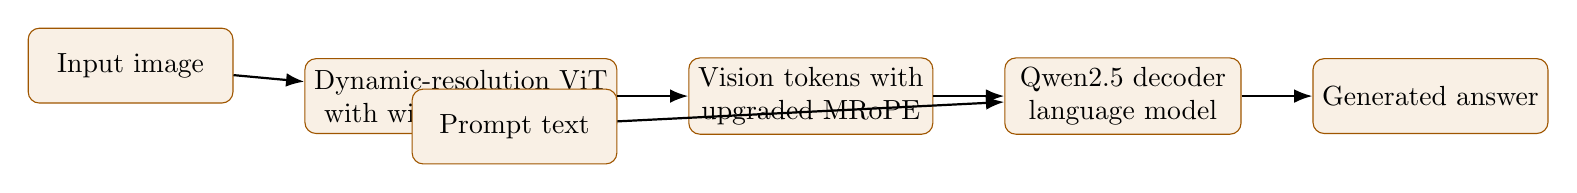
\begin{tikzpicture}[node distance=1.4cm and 0.9cm,>=Latex]
    \modelbox{qwenorange}{qvit}{Dynamic-resolution ViT\\with window attention}
    \node[left=of qvit, yshift=11pt, draw=qwenorange!80!black, fill=qwenorange!10, rounded corners, minimum width=2.6cm, minimum height=0.95cm, align=center] (qimg) {Input image};
    \node[right=of qvit, draw=qwenorange!80!black, fill=qwenorange!10, rounded corners, minimum width=3.0cm, minimum height=0.95cm, align=center] (qrope) {Vision tokens with\\upgraded MRoPE};
    \node[left=of qrope, yshift=-11pt, draw=qwenorange!80!black, fill=qwenorange!10, rounded corners, minimum width=2.6cm, minimum height=0.95cm, align=center] (qtext) {Prompt text};
    \node[right=of qrope, draw=qwenorange!80!black, fill=qwenorange!10, rounded corners, minimum width=3.0cm, minimum height=0.95cm, align=center] (qllm) {Qwen2.5 decoder\\language model};
    \node[right=of qllm, draw=qwenorange!80!black, fill=qwenorange!10, rounded corners, minimum width=2.6cm, minimum height=0.95cm, align=center] (qout) {Generated answer};

    \draw[->,thick] (qimg) -- (qvit);
    \draw[->,thick] (qvit) -- (qrope);
    \draw[->,thick] (qrope) -- (qllm);
    \draw[->,thick] (qtext) -- (qllm);
    \draw[->,thick] (qllm) -- (qout);
\end{tikzpicture}
\caption{High-level Qwen2.5-VL pipeline reflected in the repo's \texttt{qwen25-vl} wrapper.}
\end{figure}

\section{Why The Scores Separate}
\subsection{Why GPT-4.1 finishes first overall}
The easiest way to say it is that \texttt{gpt-4.1} looks like the most \emph{general-purpose polished} system of the three. It does not dominate every family, but it does the fewest obviously weak things. In the saved comparison outputs, it is strongest on labeling and edges out the field overall on average score.

That pattern makes sense. Labeling benchmarks reward robust visual recognition, careful prompt following, and stable output formatting. Proprietary frontier systems usually have an advantage here because they are trained at larger scale, tuned heavily for instruction reliability, and optimized around product use cases where small formatting failures matter.

There is also a softer point: \texttt{gpt-4.1} appears to degrade gracefully. It may not win every benchmark outright, but it avoids the sharp collapses that drag down open-weight models when the prompt format, class granularity, or image distribution shifts.

\subsection{Why Qwen2.5-VL wins more individual benchmarks}
\texttt{qwen25-vl} has the best mean rank and the most first-place finishes. That usually means the model has a high ceiling and a strong multimodal alignment stack, even if it is a little less even across the whole suite than \texttt{gpt-4.1}.

The family breakdown supports that reading. Qwen is best on captioning and remains strong everywhere else. Captioning tends to reward rich image grounding, fluent generation, and the ability to turn visual details into natural text without sounding formulaic. That is exactly the sort of behavior that a stronger native multimodal design can improve.

Its public design choices also line up with the observed results. A better vision encoder path, dynamic resolution handling, and stronger positional treatment should help when the image itself carries a lot of the useful information and the model needs to preserve more of that structure before generation.

\subsection{Why LLaVA-7B stays close but does not quite lead}
\texttt{llava-7b} is the most interpretable model of the three in the sense that its strengths and weaknesses look like what you would expect from the architecture. It is built from a good vision encoder plus a good language model joined by a projector. That design works, and it works surprisingly well, but it still has a bottleneck at the interface between vision features and the language backbone.

In plain English, LLaVA often feels like a strong text model that has learned to look, rather than a model built around vision from the start. That is not meant as a criticism. It is exactly why it can be so competitive for its size. But it also helps explain why it lands a bit behind \texttt{gpt-4.1} and \texttt{qwen25-vl} when the task needs very precise visual grounding or more robust multimodal reasoning across varied benchmark styles.

\subsection{Why the ranking changes by task family}
The ranking changes because the benchmark families ask for different kinds of competence:
\begin{itemize}[leftmargin=*]
    \item Captioning rewards expressive grounded generation. Qwen does best here, with LLaVA close behind.
    \item Labeling rewards disciplined classification behavior and clean mapping from image to exact label inventory. GPT-4.1 is clearly best here.
    \item Detection is unstable for all three because this benchmark is both format-sensitive and spatially demanding. GPT-4.1 and Qwen are competitive; LLaVA collapses harder.
    \item QA in this suite is noisy enough that the differences should not be over-read, but GPT-4.1 is not the leader there and Qwen remains stronger overall than the raw QA row alone would suggest.
\end{itemize}

\section{A Note About Speed}
The telemetry should be read carefully. In the comparison output, \texttt{llava-7b} and \texttt{gpt-4.1} are the fastest of the three, while \texttt{qwen25-vl} is still fairly quick:

\begin{table}[H]
\centering
\caption{Telemetry from \texttt{comparison/output/telemetry\_model\_summary.csv}.}
\begin{tabular}{>{\ttfamily}lrrr}
\toprule
Model & Mean wall-clock (s) & Mean generation (s) & Peak CPU RAM (GiB) \\
\midrule
llava-7b & 1.19 & 1.11 & 4.34 \\
gpt-4.1 & 1.42 & 1.35 & 4.54 \\
qwen25-vl & 2.70 & 2.58 & 4.03 \\
\bottomrule
\end{tabular}
\end{table}

\noindent
That said, this is not a perfectly apples-to-apples systems benchmark. \texttt{gpt-4.1} is called through a remote API, so the local machine is not doing the same kind of work it is doing for the two open-weight models. The speed numbers are still useful operationally, but they are not pure model-efficiency measurements.

\section{Pairwise Reading}
The pairwise win table says something subtle and important:
\begin{itemize}[leftmargin=*]
    \item \texttt{qwen25-vl} beats \texttt{llava-7b} on 11 of 21 shared benchmarks.
    \item \texttt{qwen25-vl} beats \texttt{gpt-4.1} on 8 of 21, while \texttt{gpt-4.1} beats Qwen on 7 of 21, with 6 ties.
    \item \texttt{llava-7b} beats \texttt{gpt-4.1} on 7 of 21, with 8 ties.
\end{itemize}

\noindent
So this is not a clean ladder where one model simply dominates the next. It is more like this:
\begin{itemize}[leftmargin=*]
    \item \texttt{gpt-4.1} is the safest overall pick.
    \item \texttt{qwen25-vl} is the sharpest multimodal specialist among the three.
    \item \texttt{llava-7b} is credible enough that any serious evaluation should keep it in the room.
\end{itemize}

\section{Practical Takeaways}
If I had to summarize the three models in ordinary language:
\begin{itemize}[leftmargin=*]
    \item \texttt{gpt-4.1} is the one I would trust most when I want the fewest surprises.
    \item \texttt{qwen25-vl} is the one I would reach for when image grounding and natural visual description matter a lot.
    \item \texttt{llava-7b} is the one that proves how far a simpler open architecture can go before the more integrated multimodal systems start to pull away.
\end{itemize}

\section{Comparison Graphs}
The figures below are the graphs generated by the comparison pipeline and included here directly from \texttt{comparison/output/}. They are presented with only light commentary because the plots mostly speak for themselves.

\begin{figure}[p]
\centering
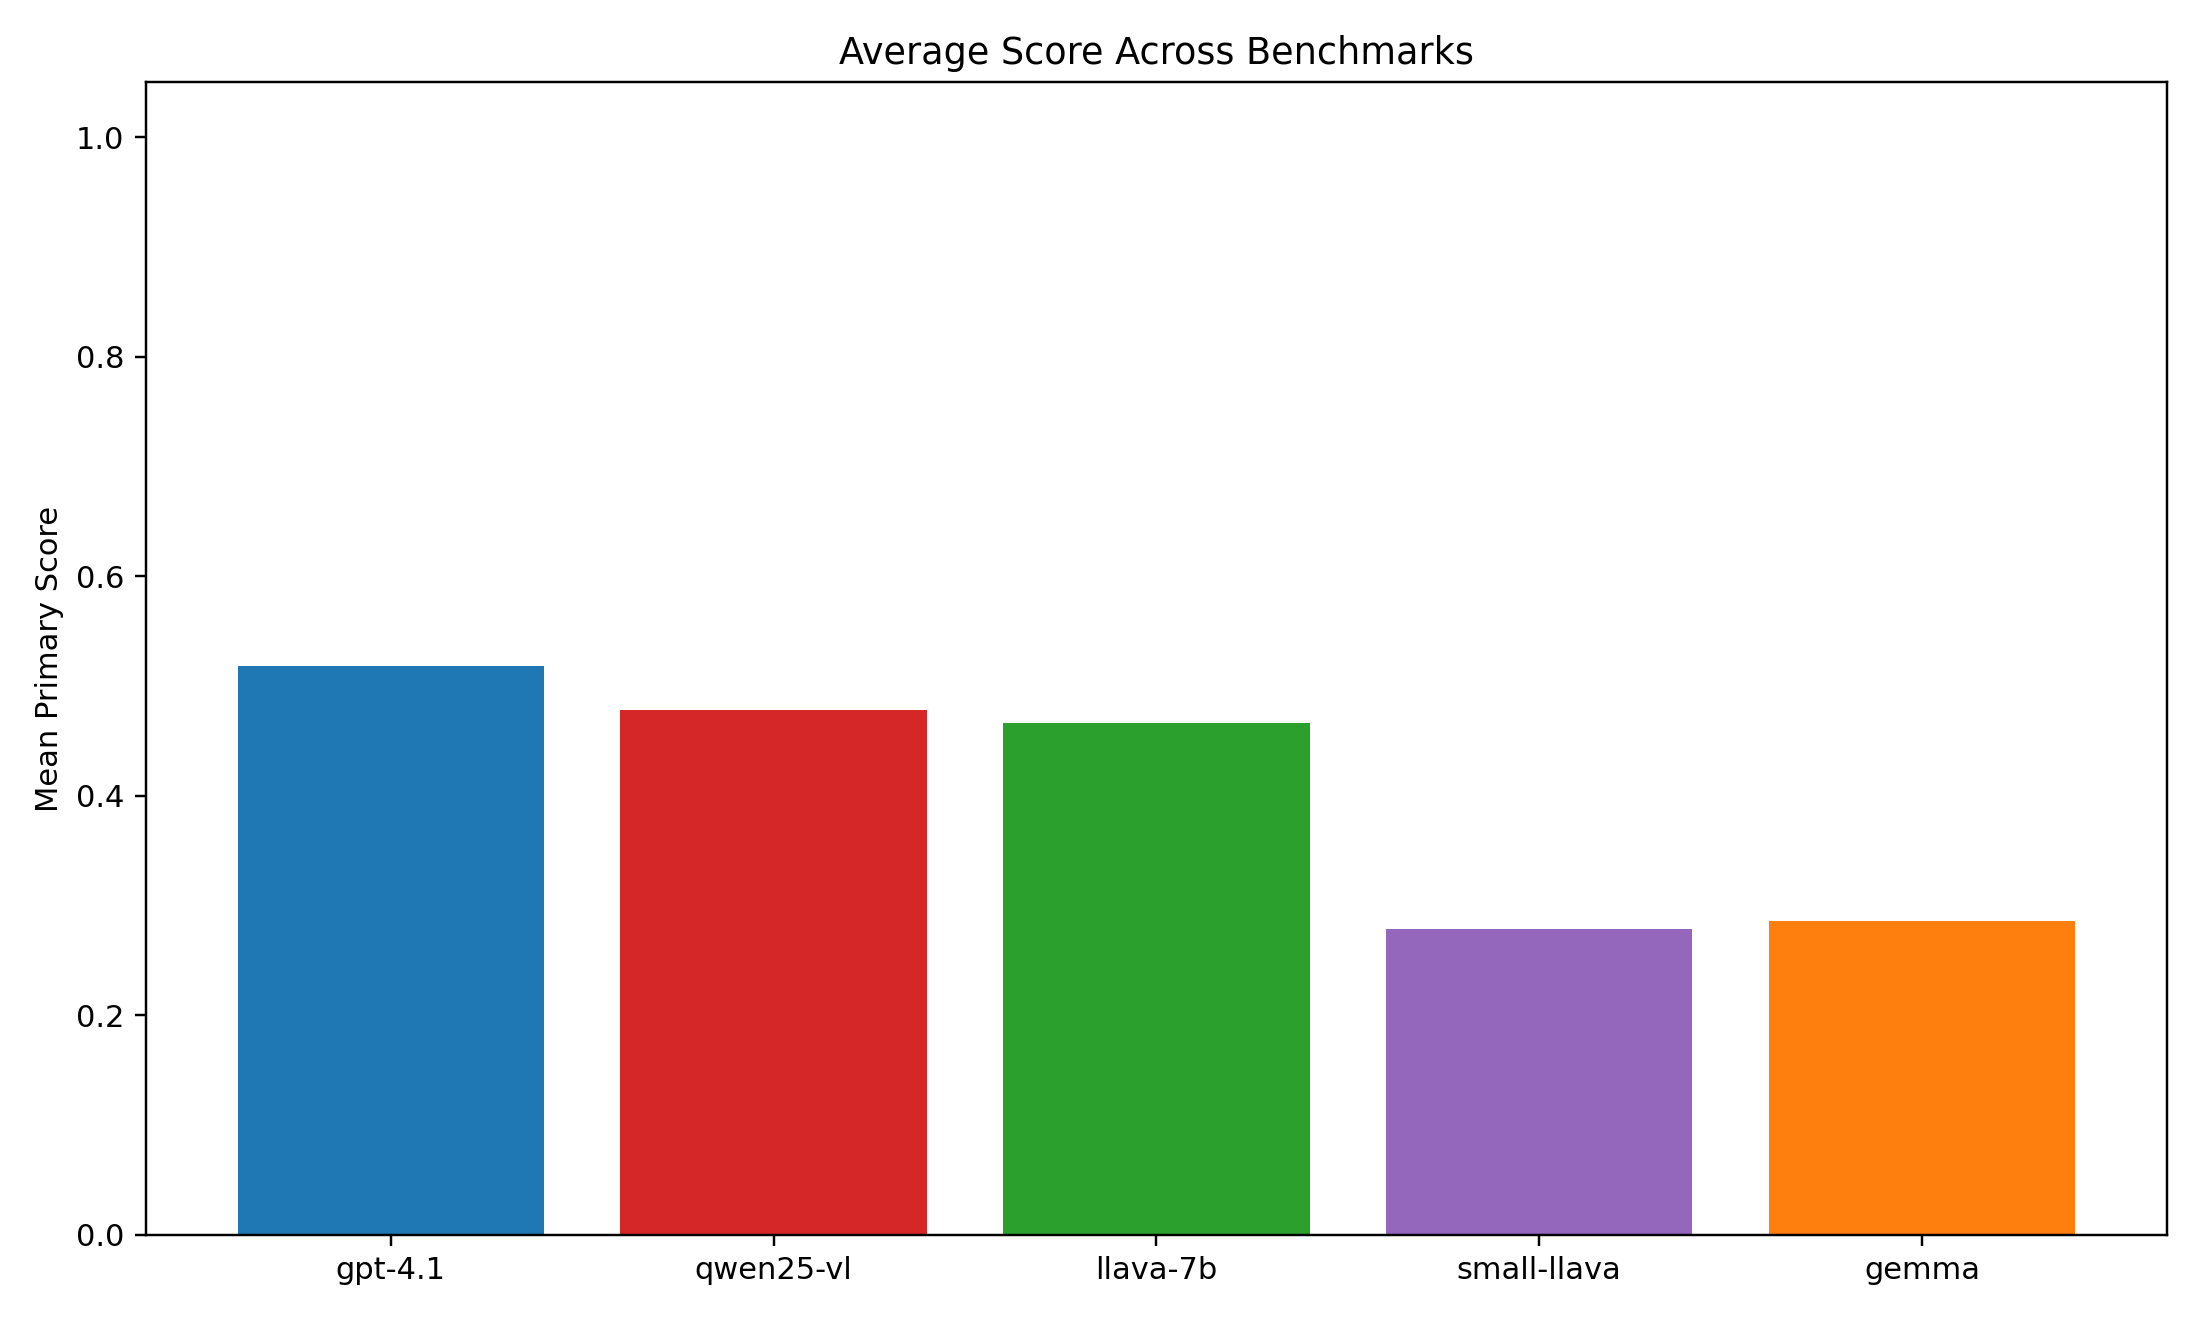
\includegraphics[width=\textwidth]{comparison/output/model_mean_scores.png}
\caption{Mean raw scores by model.}
\end{figure}

\begin{figure}[p]
\centering
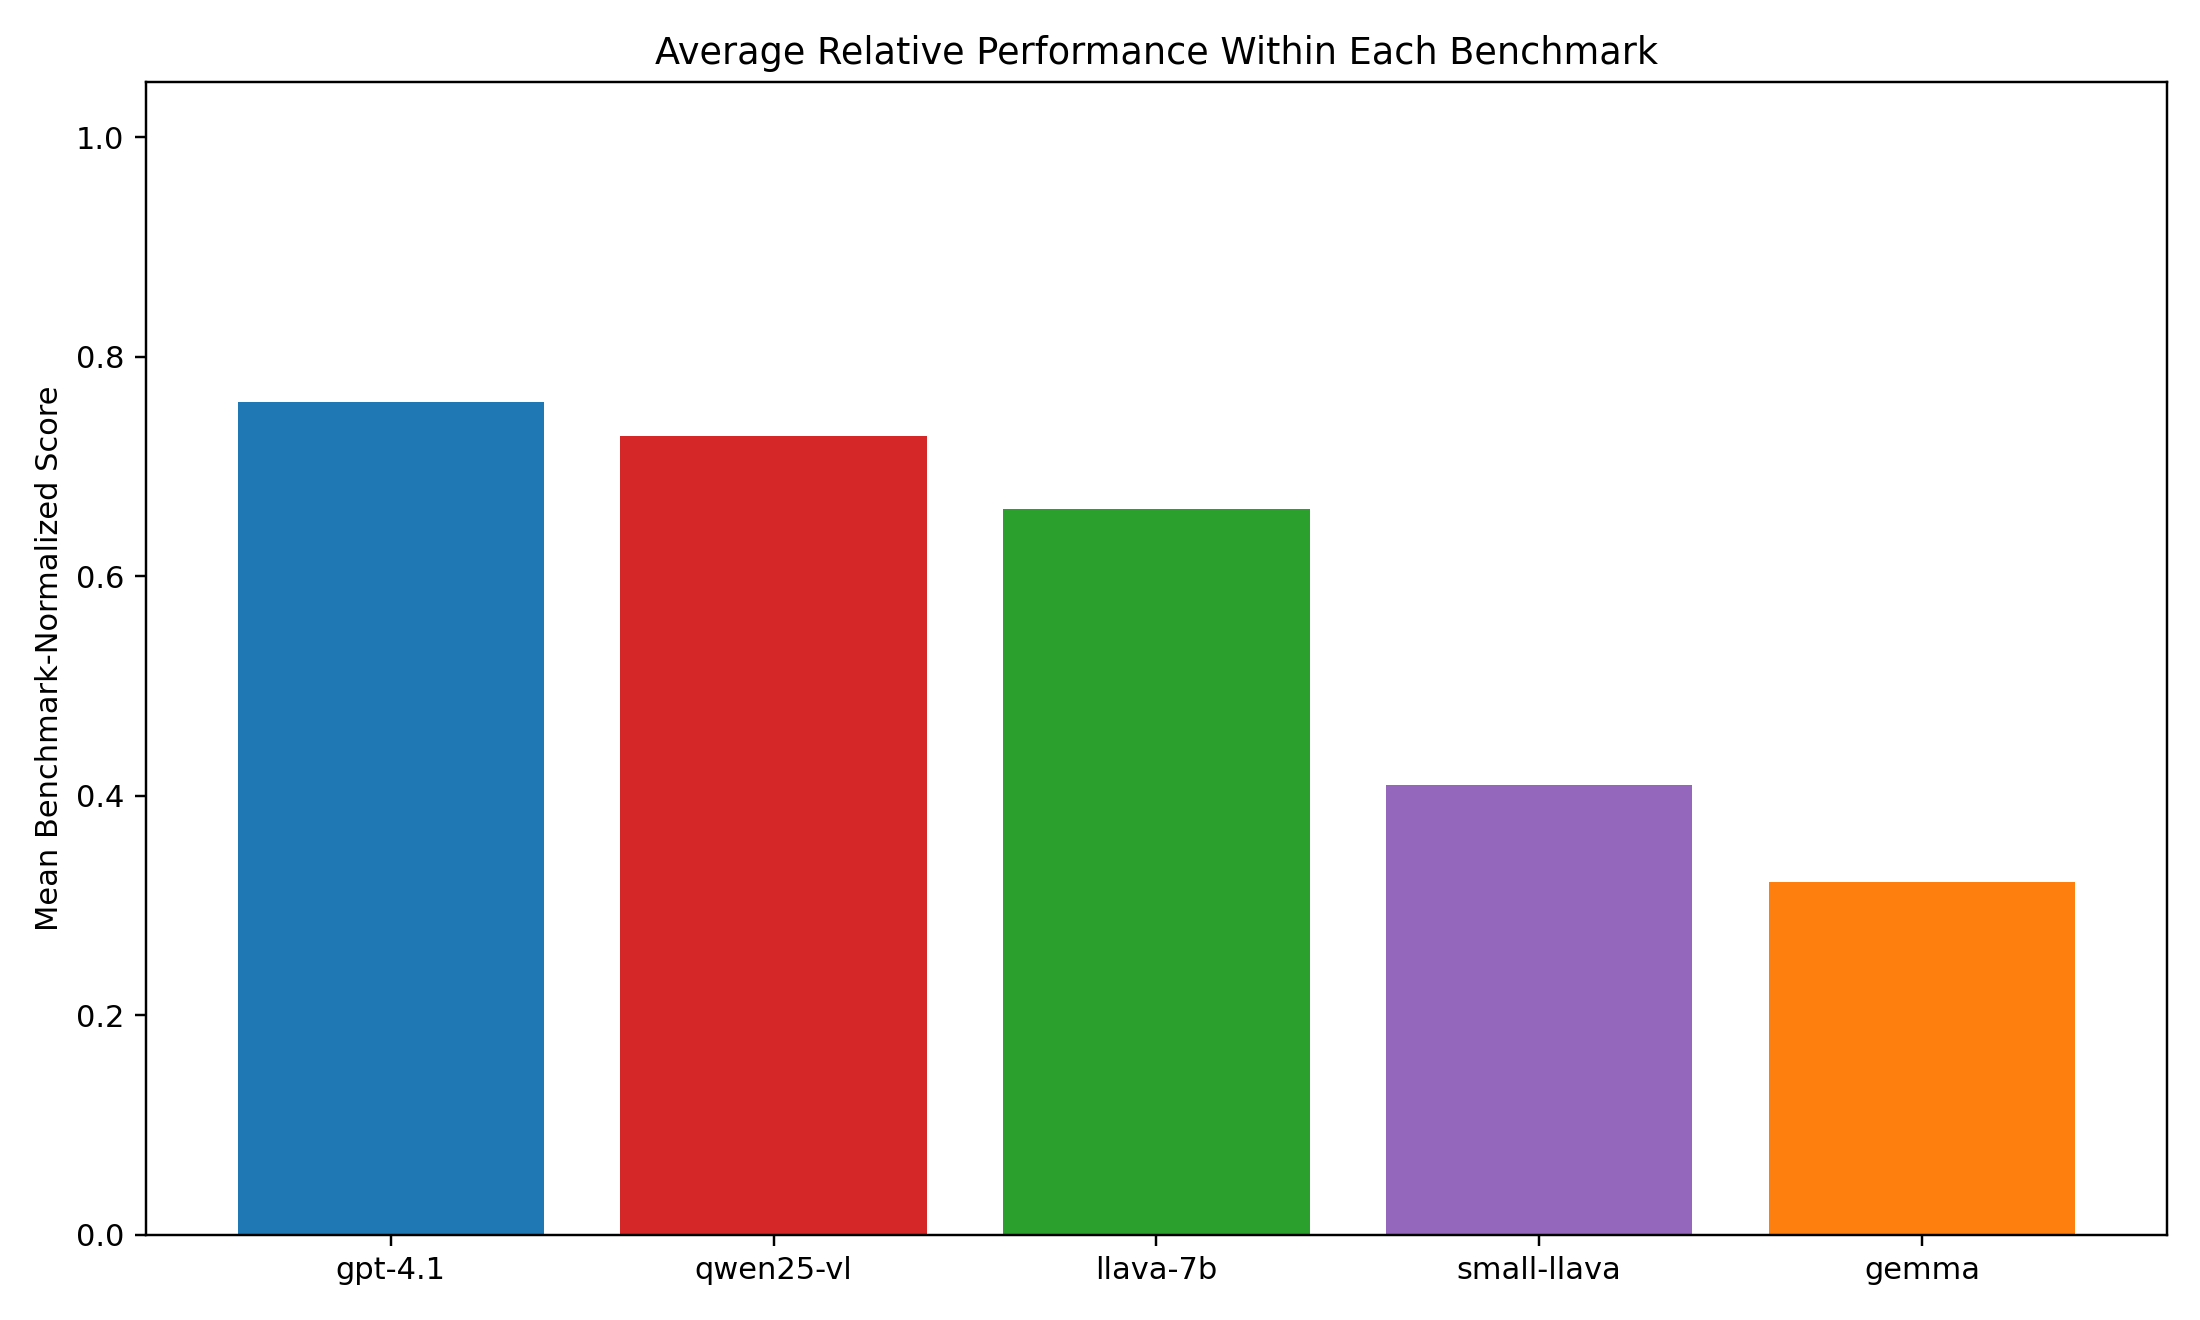
\includegraphics[width=\textwidth]{comparison/output/model_normalized_scores.png}
\caption{Mean benchmark-normalized scores by model.}
\end{figure}

\begin{figure}[p]
\centering
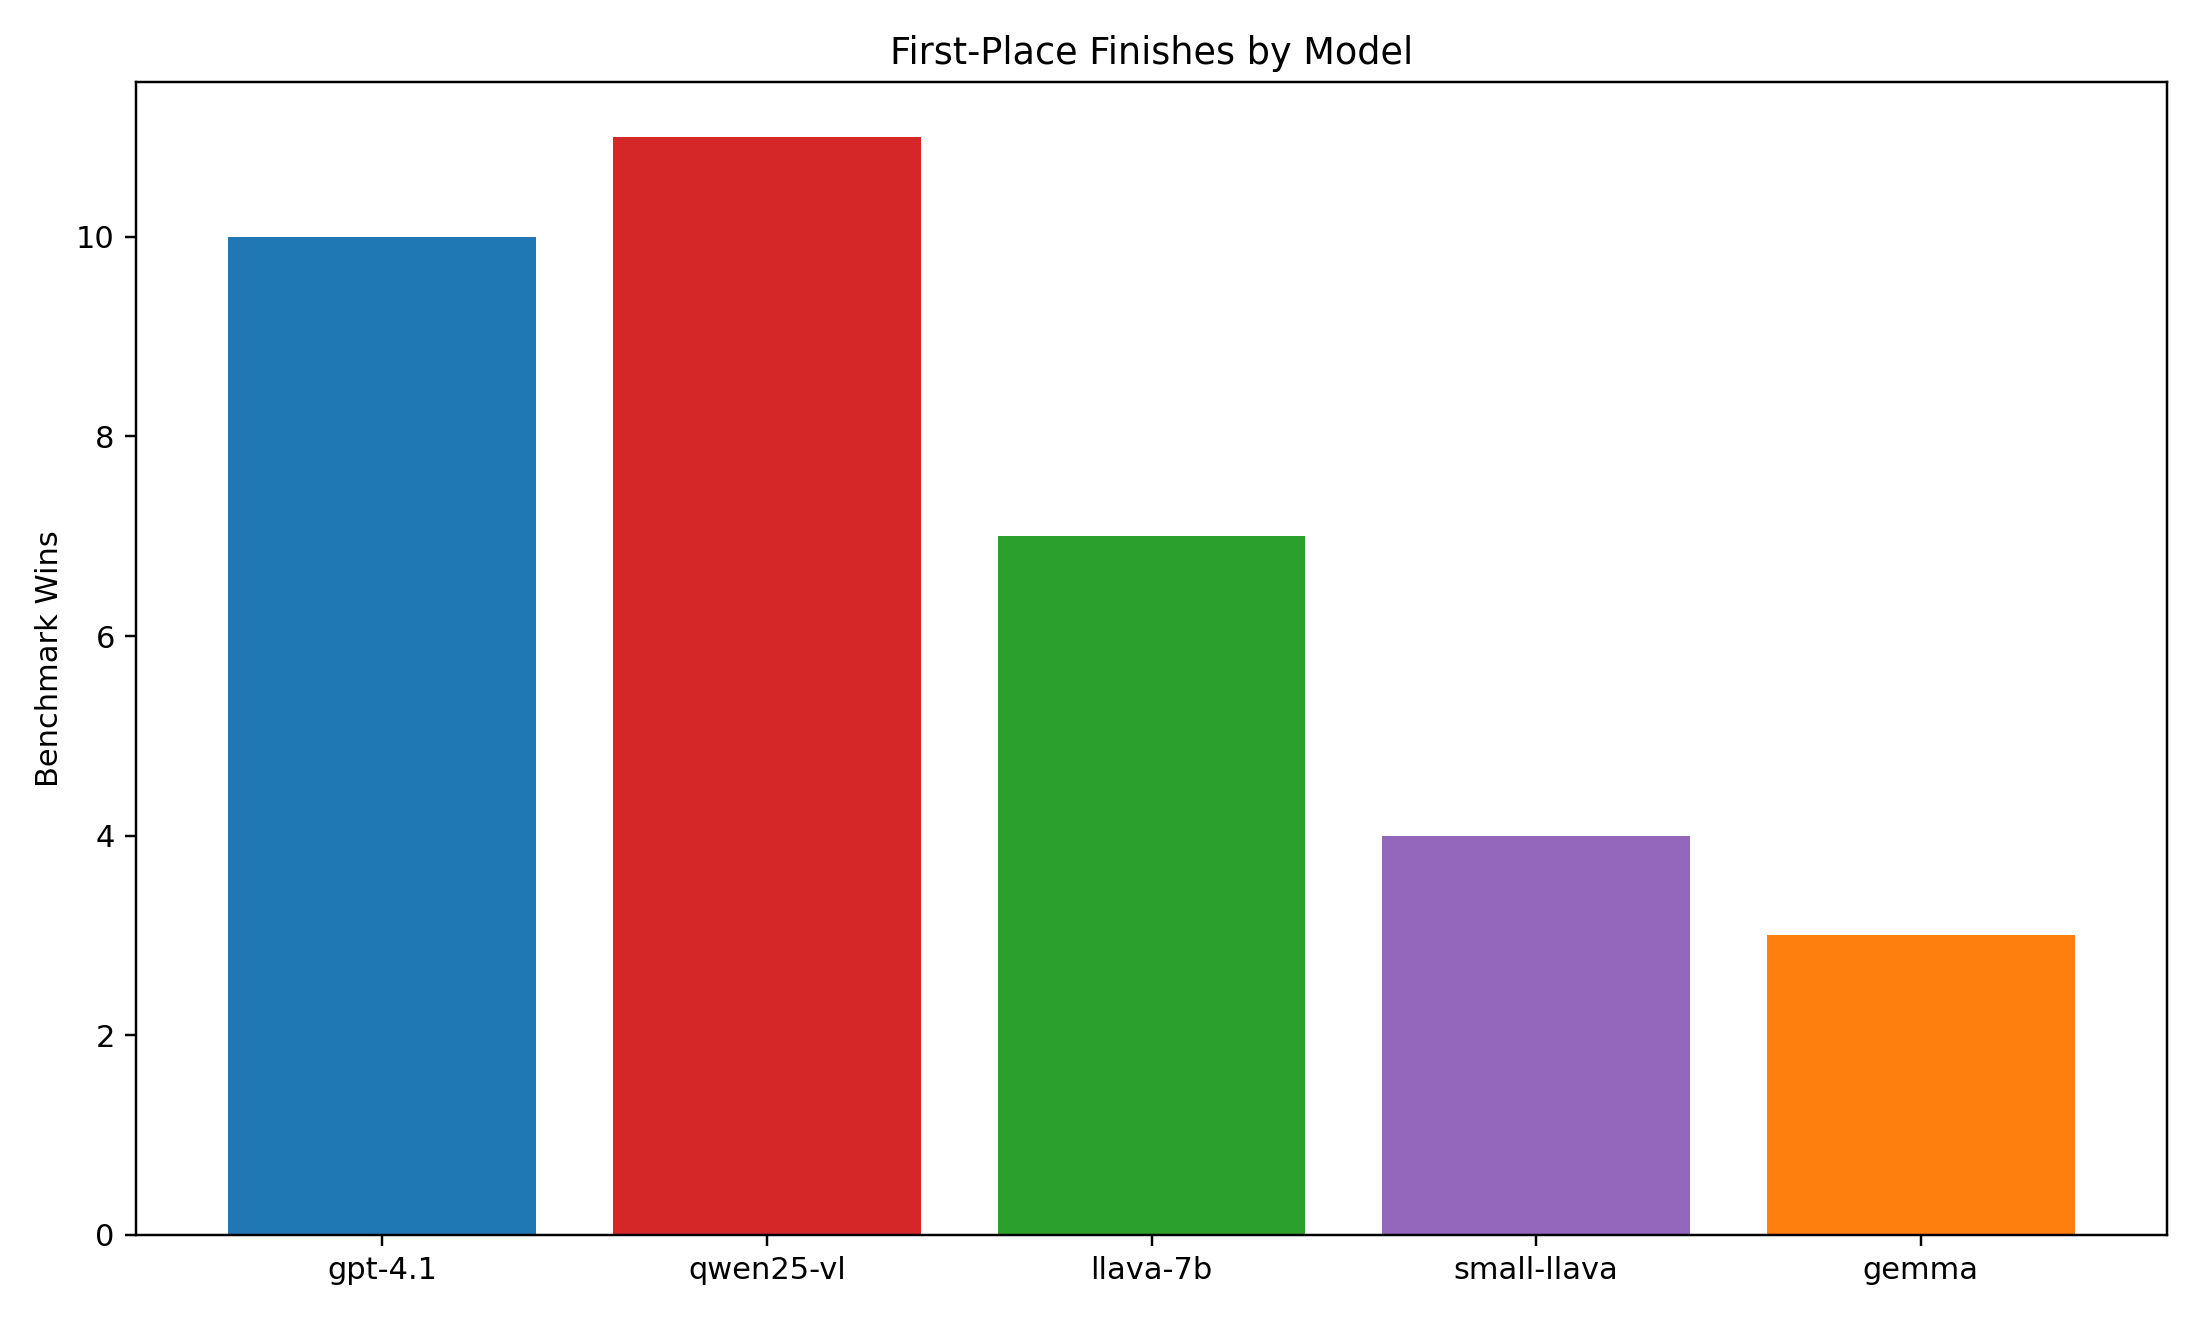
\includegraphics[width=\textwidth]{comparison/output/first_place_finishes.png}
\caption{First-place finishes by model.}
\end{figure}

\begin{figure}[p]
\centering
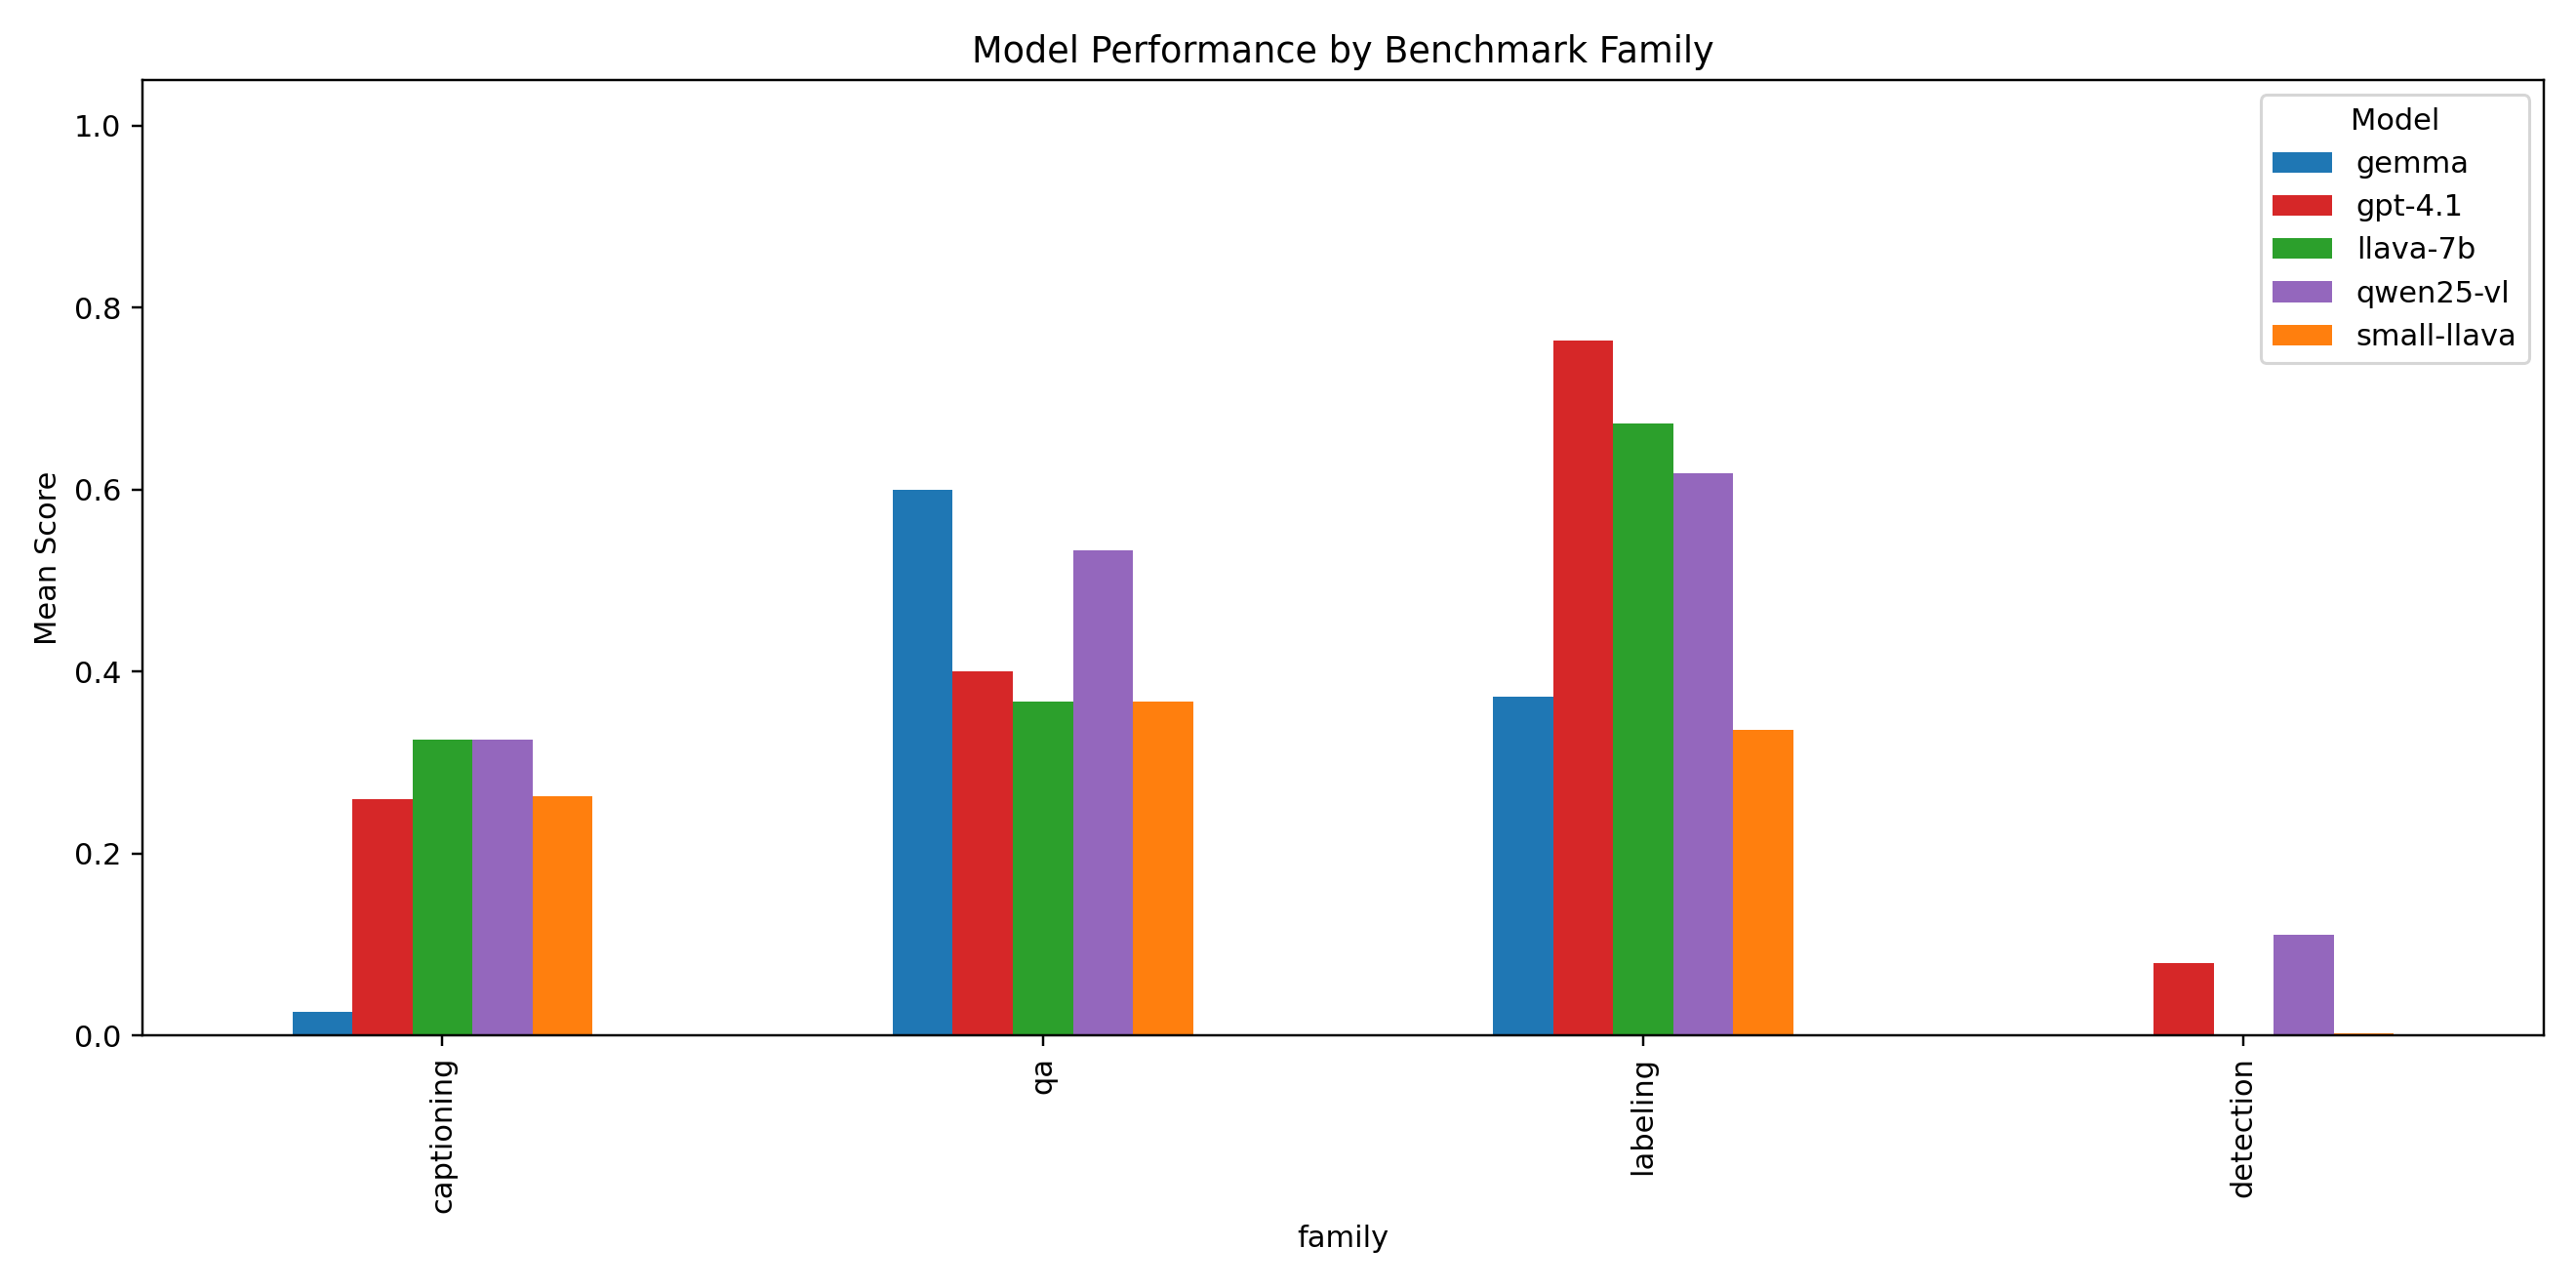
\includegraphics[width=\textwidth]{comparison/output/family_grouped_bars.png}
\caption{Grouped family comparison.}
\end{figure}

\begin{figure}[p]
\centering
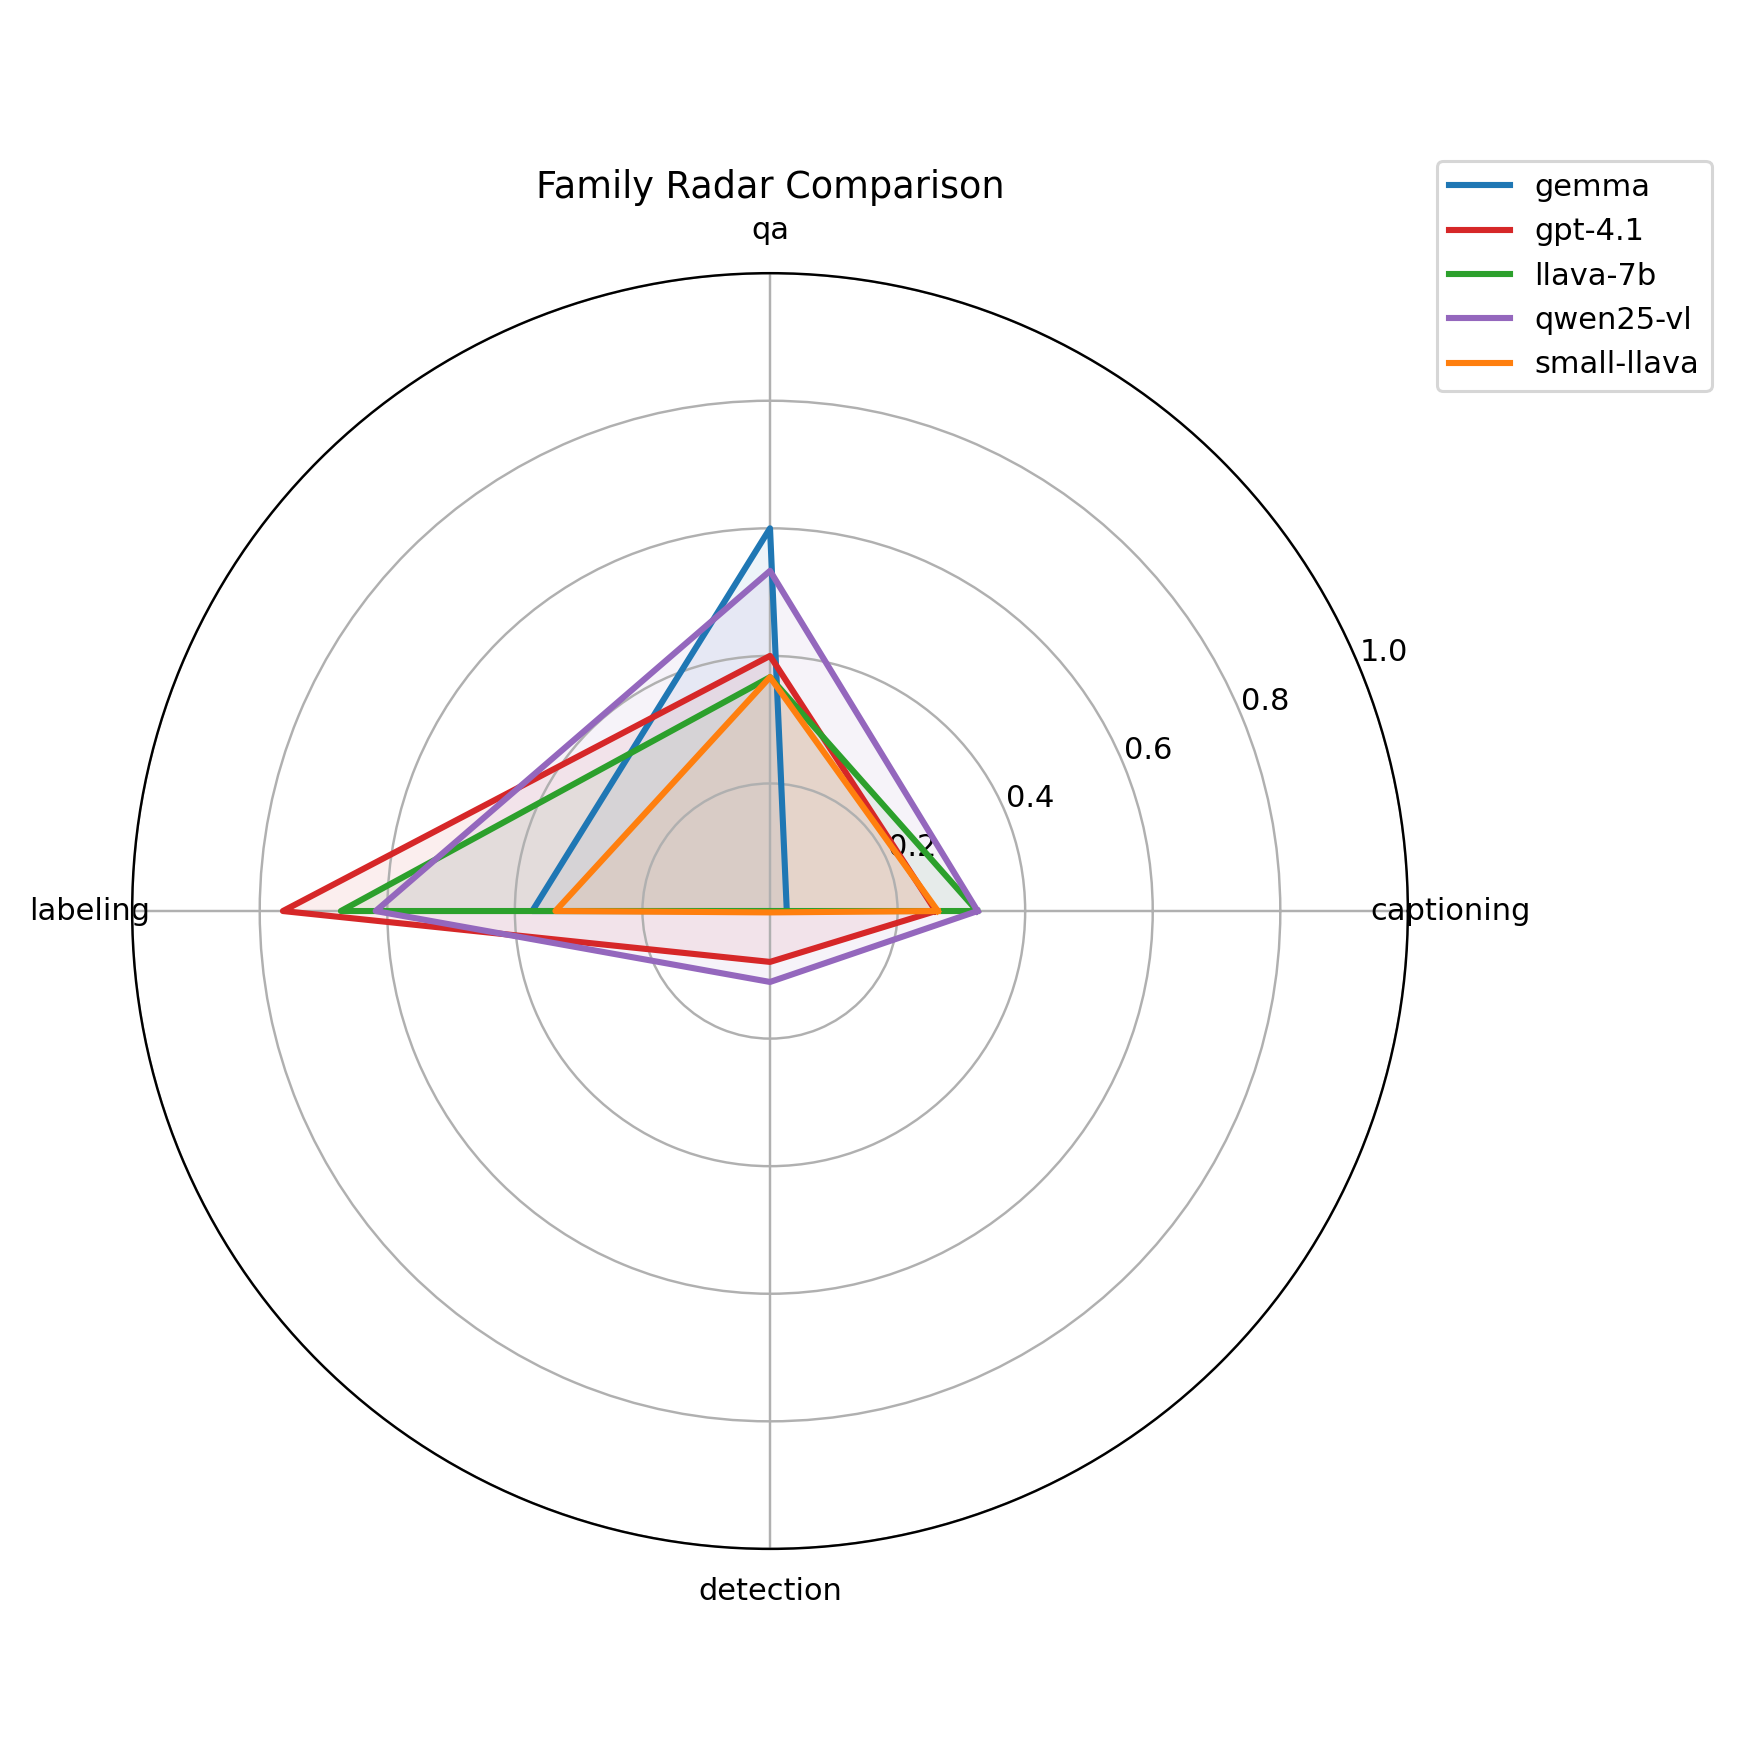
\includegraphics[width=\textwidth]{comparison/output/family_radar.png}
\caption{Family radar comparison.}
\end{figure}

\begin{figure}[p]
\centering
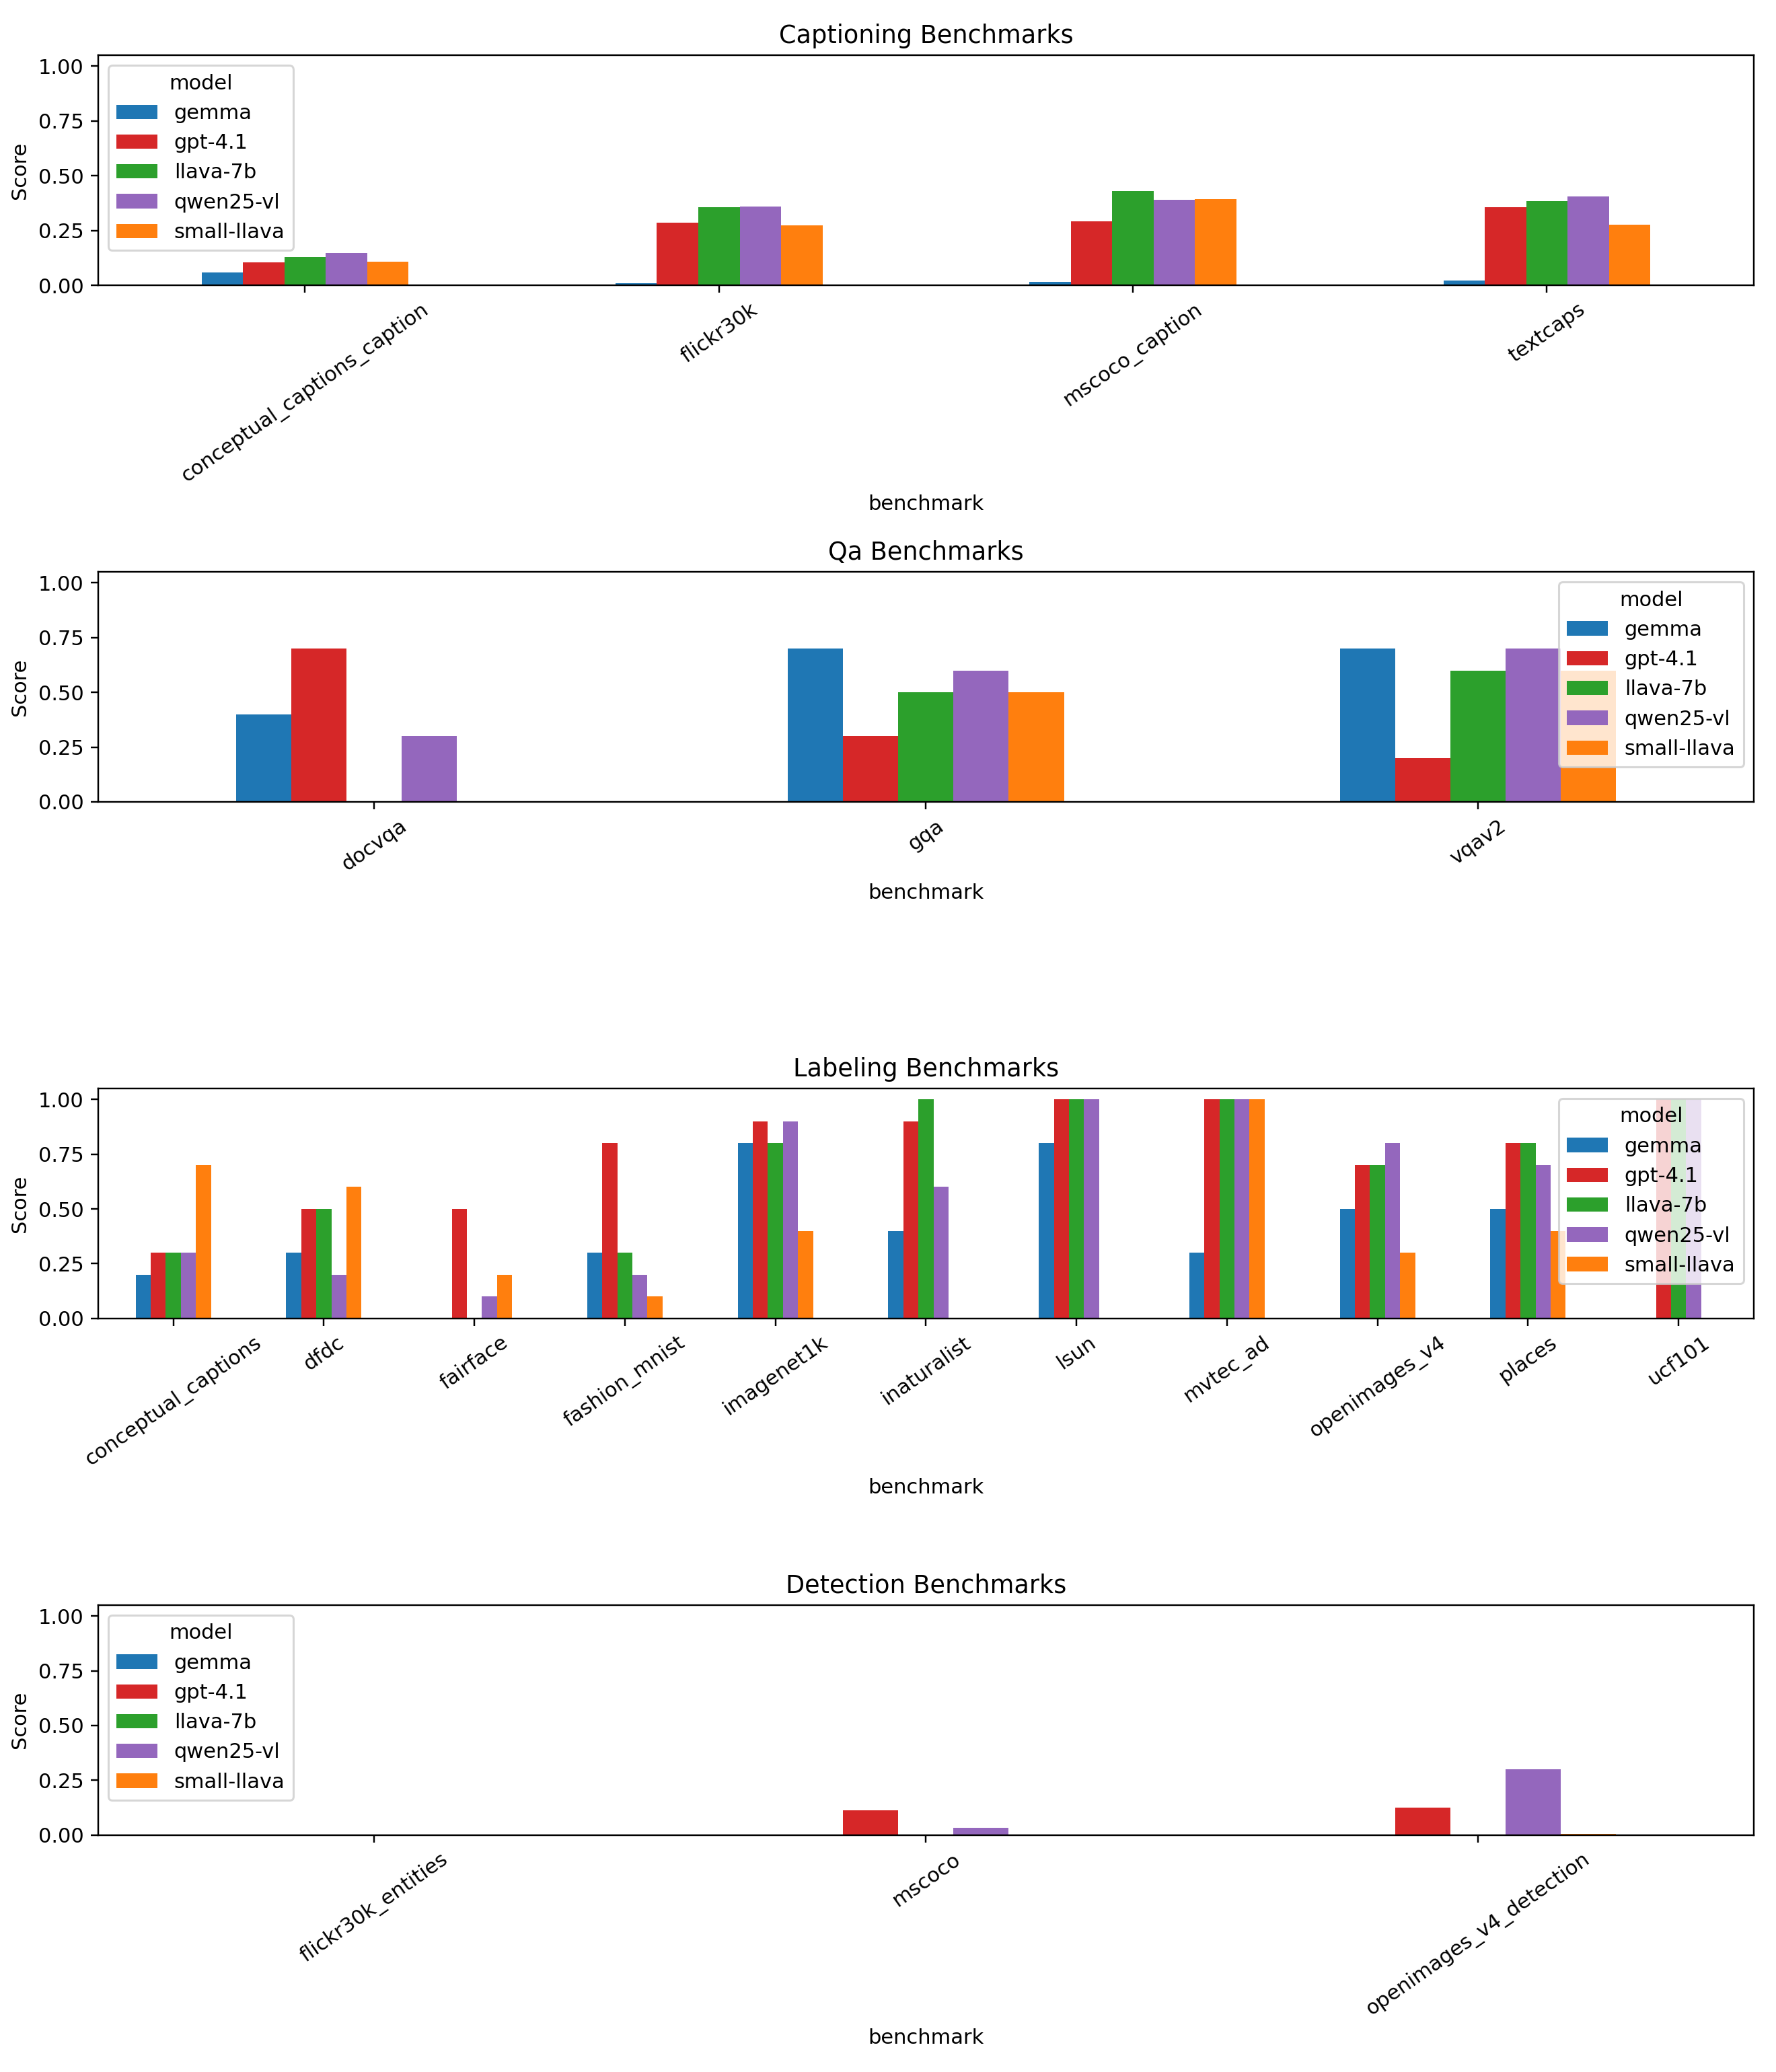
\includegraphics[width=\textwidth]{comparison/output/family_small_multiples.png}
\caption{Family small multiples.}
\end{figure}

\begin{figure}[p]
\centering
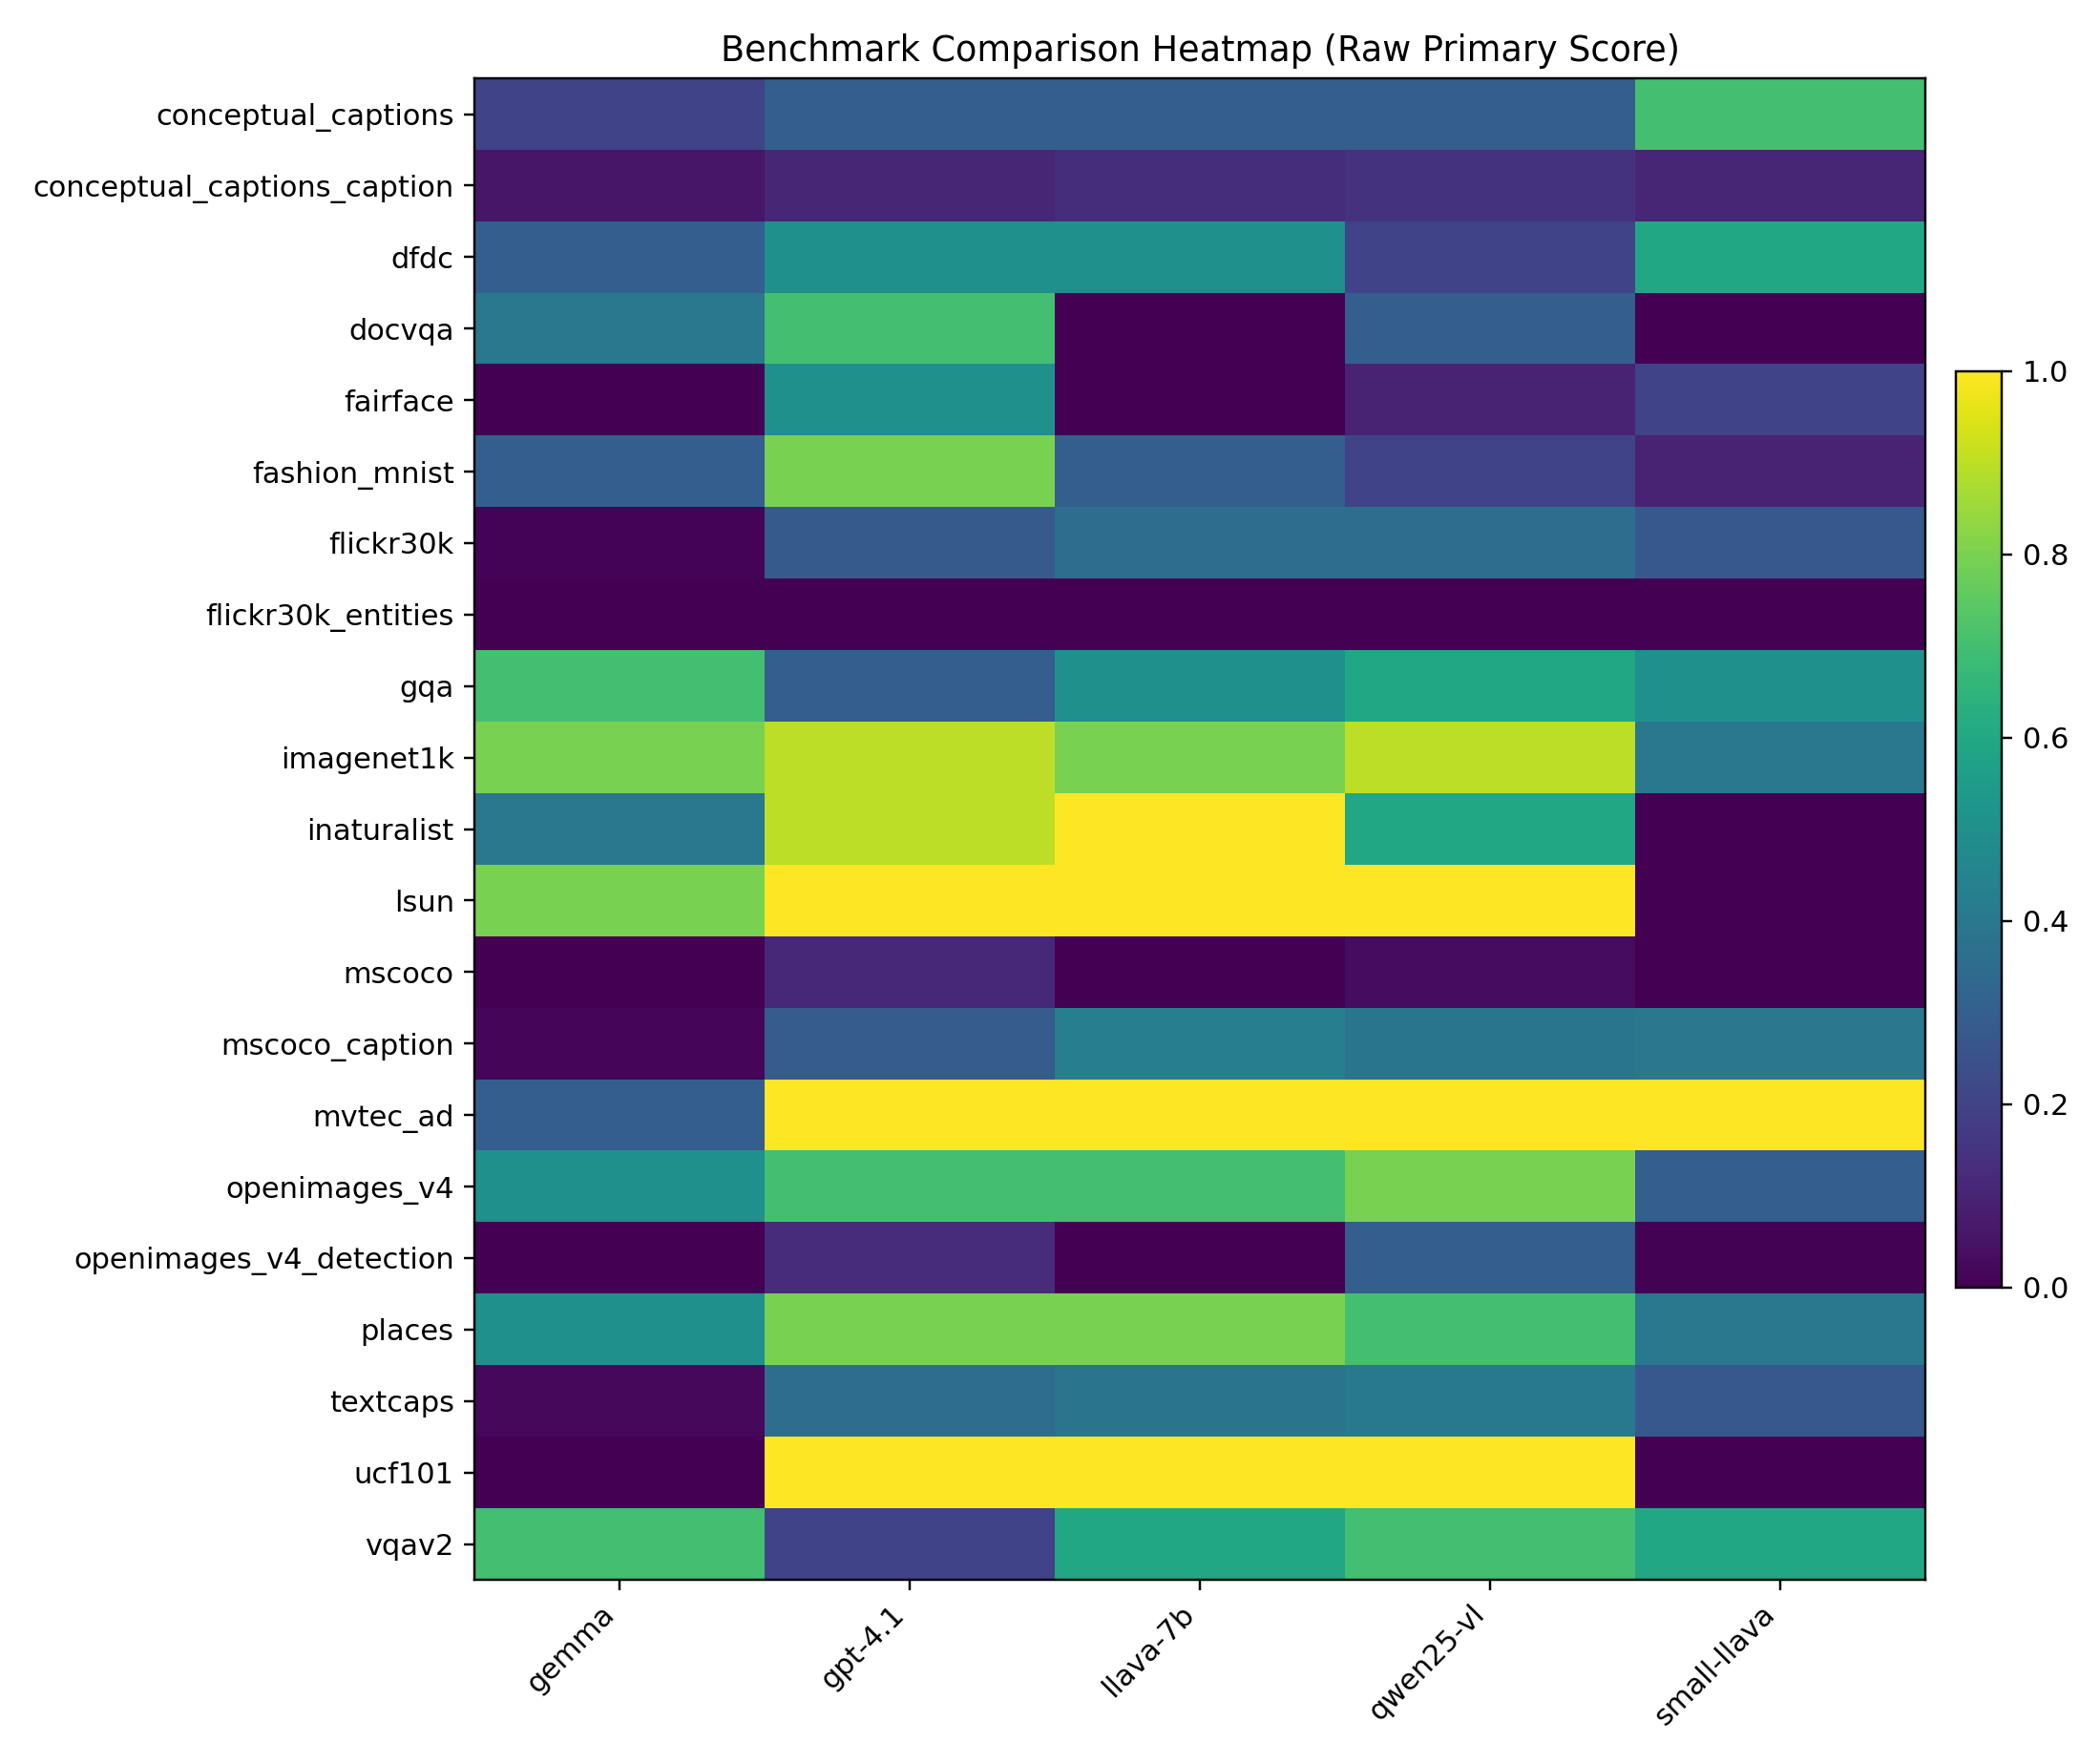
\includegraphics[width=\textwidth]{comparison/output/score_heatmap_raw.png}
\caption{Raw benchmark score heatmap.}
\end{figure}

\begin{figure}[p]
\centering
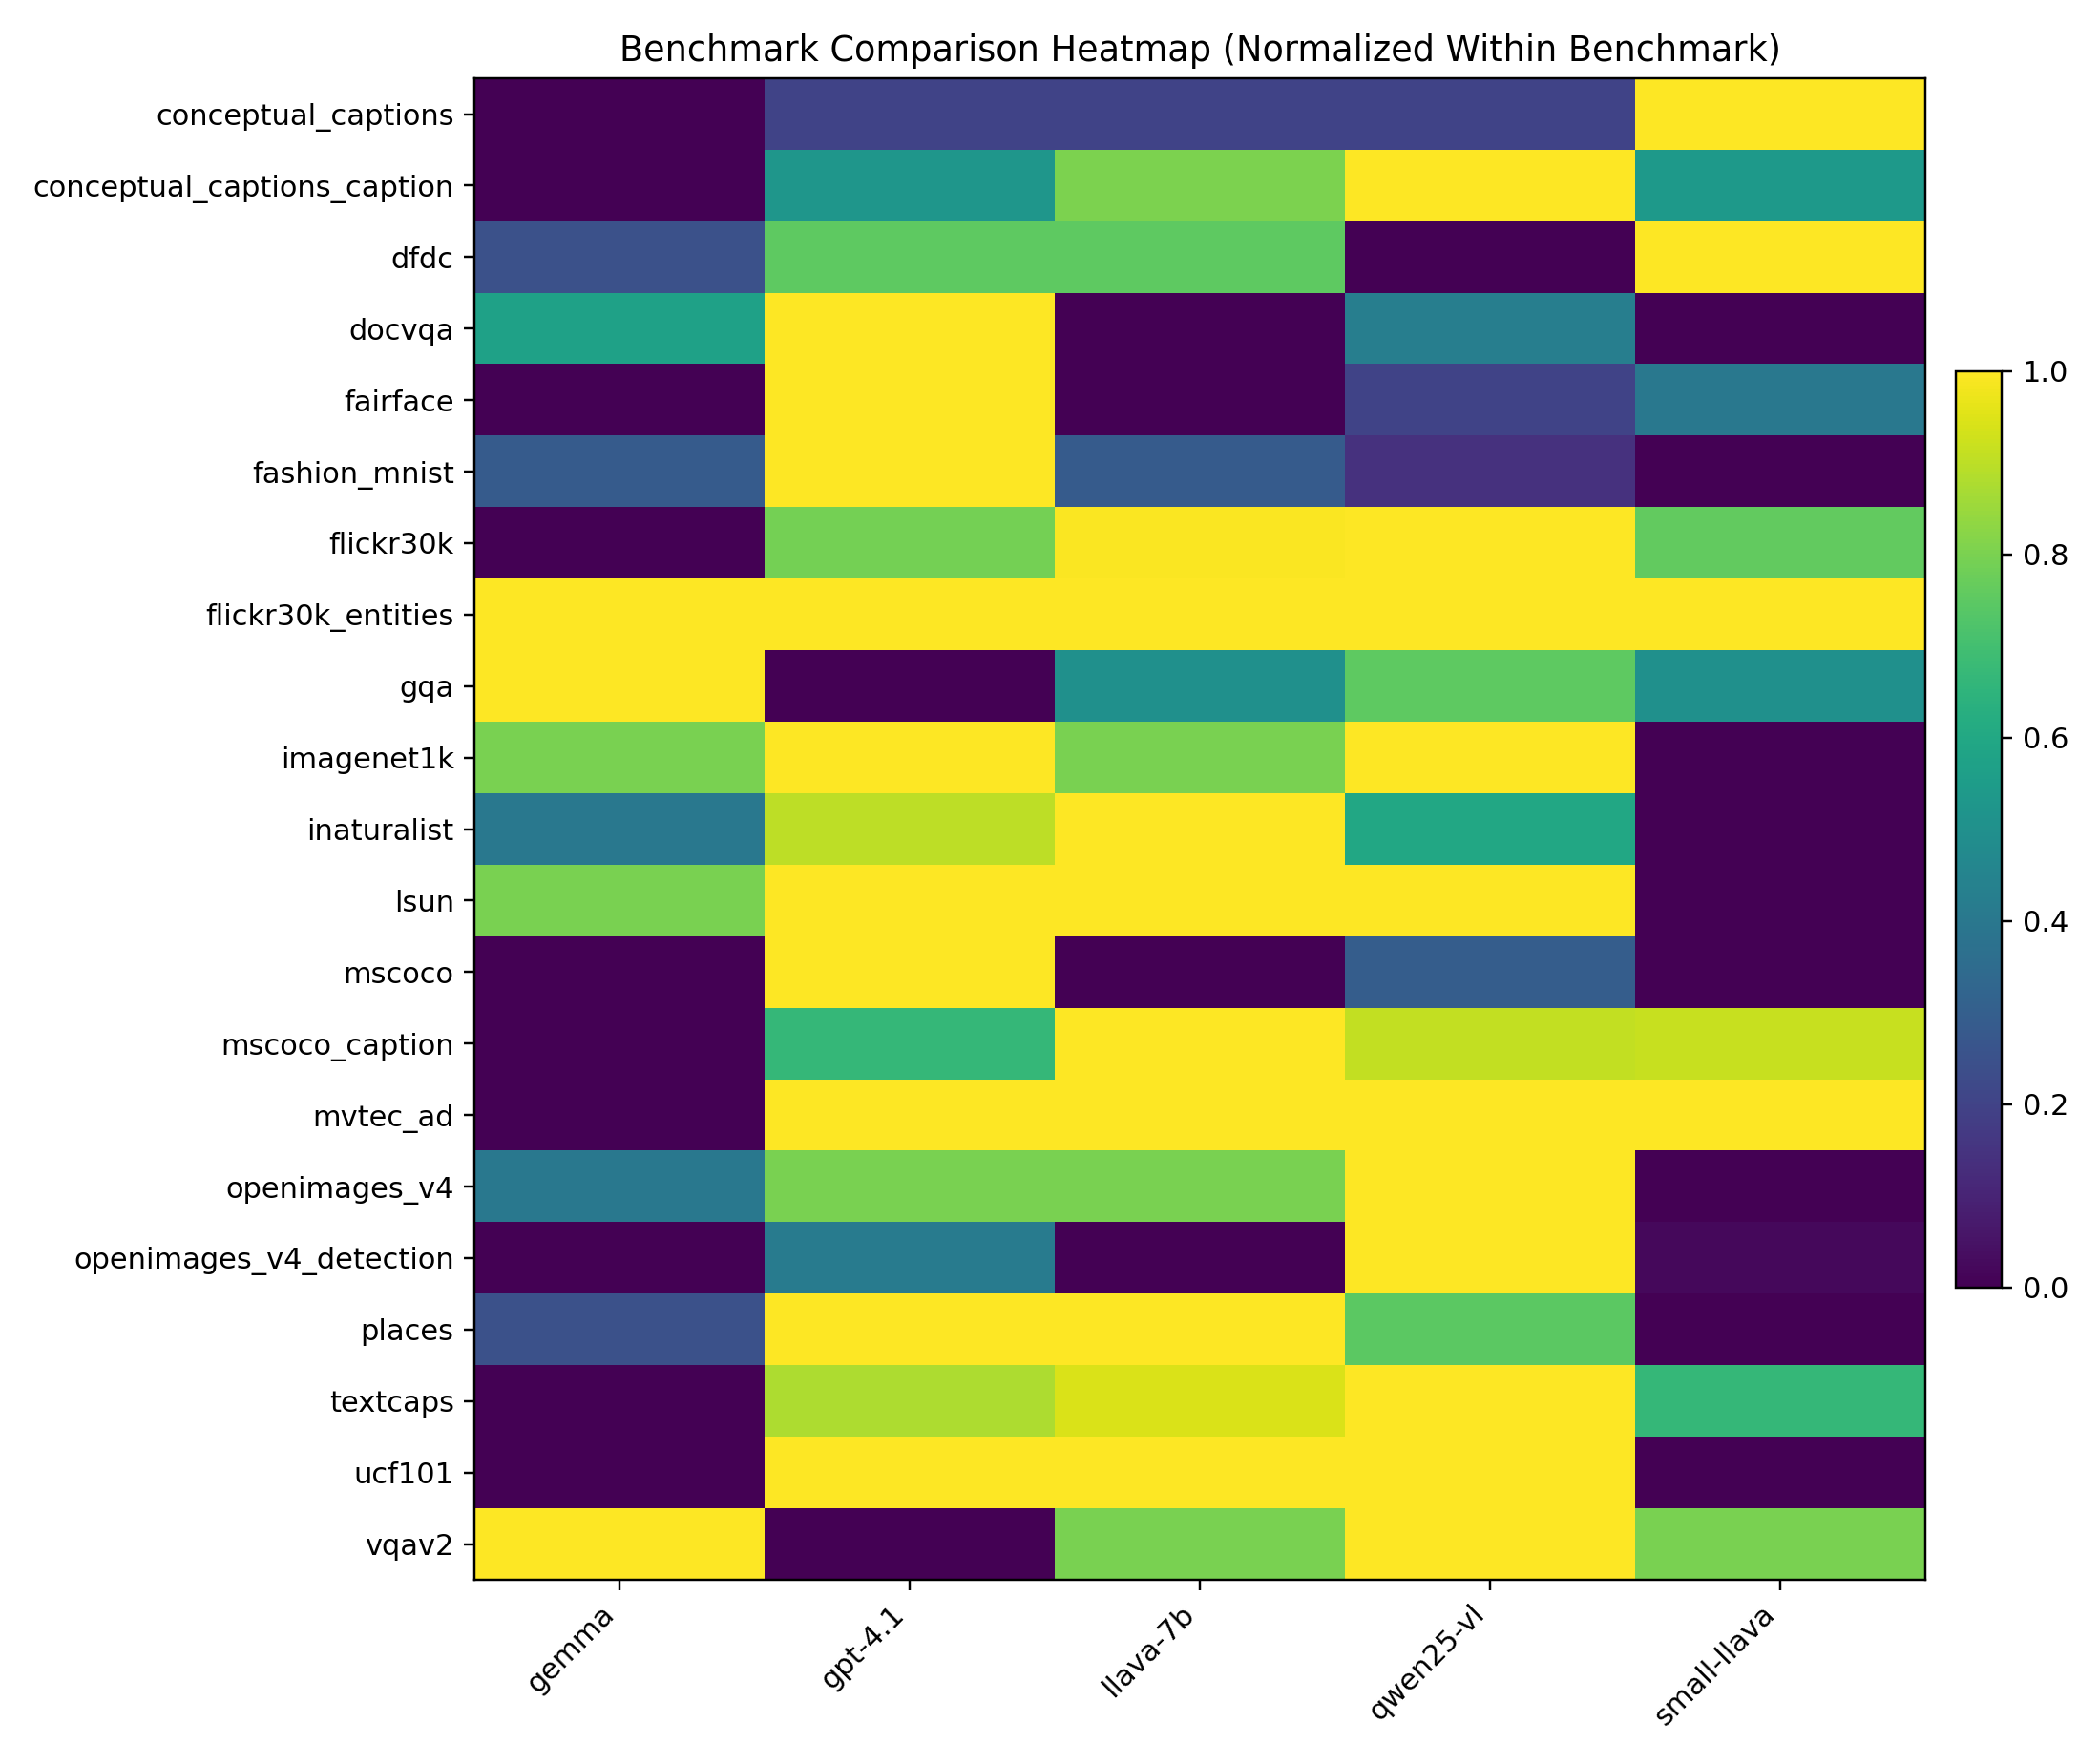
\includegraphics[width=\textwidth]{comparison/output/score_heatmap_normalized.png}
\caption{Normalized benchmark score heatmap.}
\end{figure}

\begin{figure}[p]
\centering
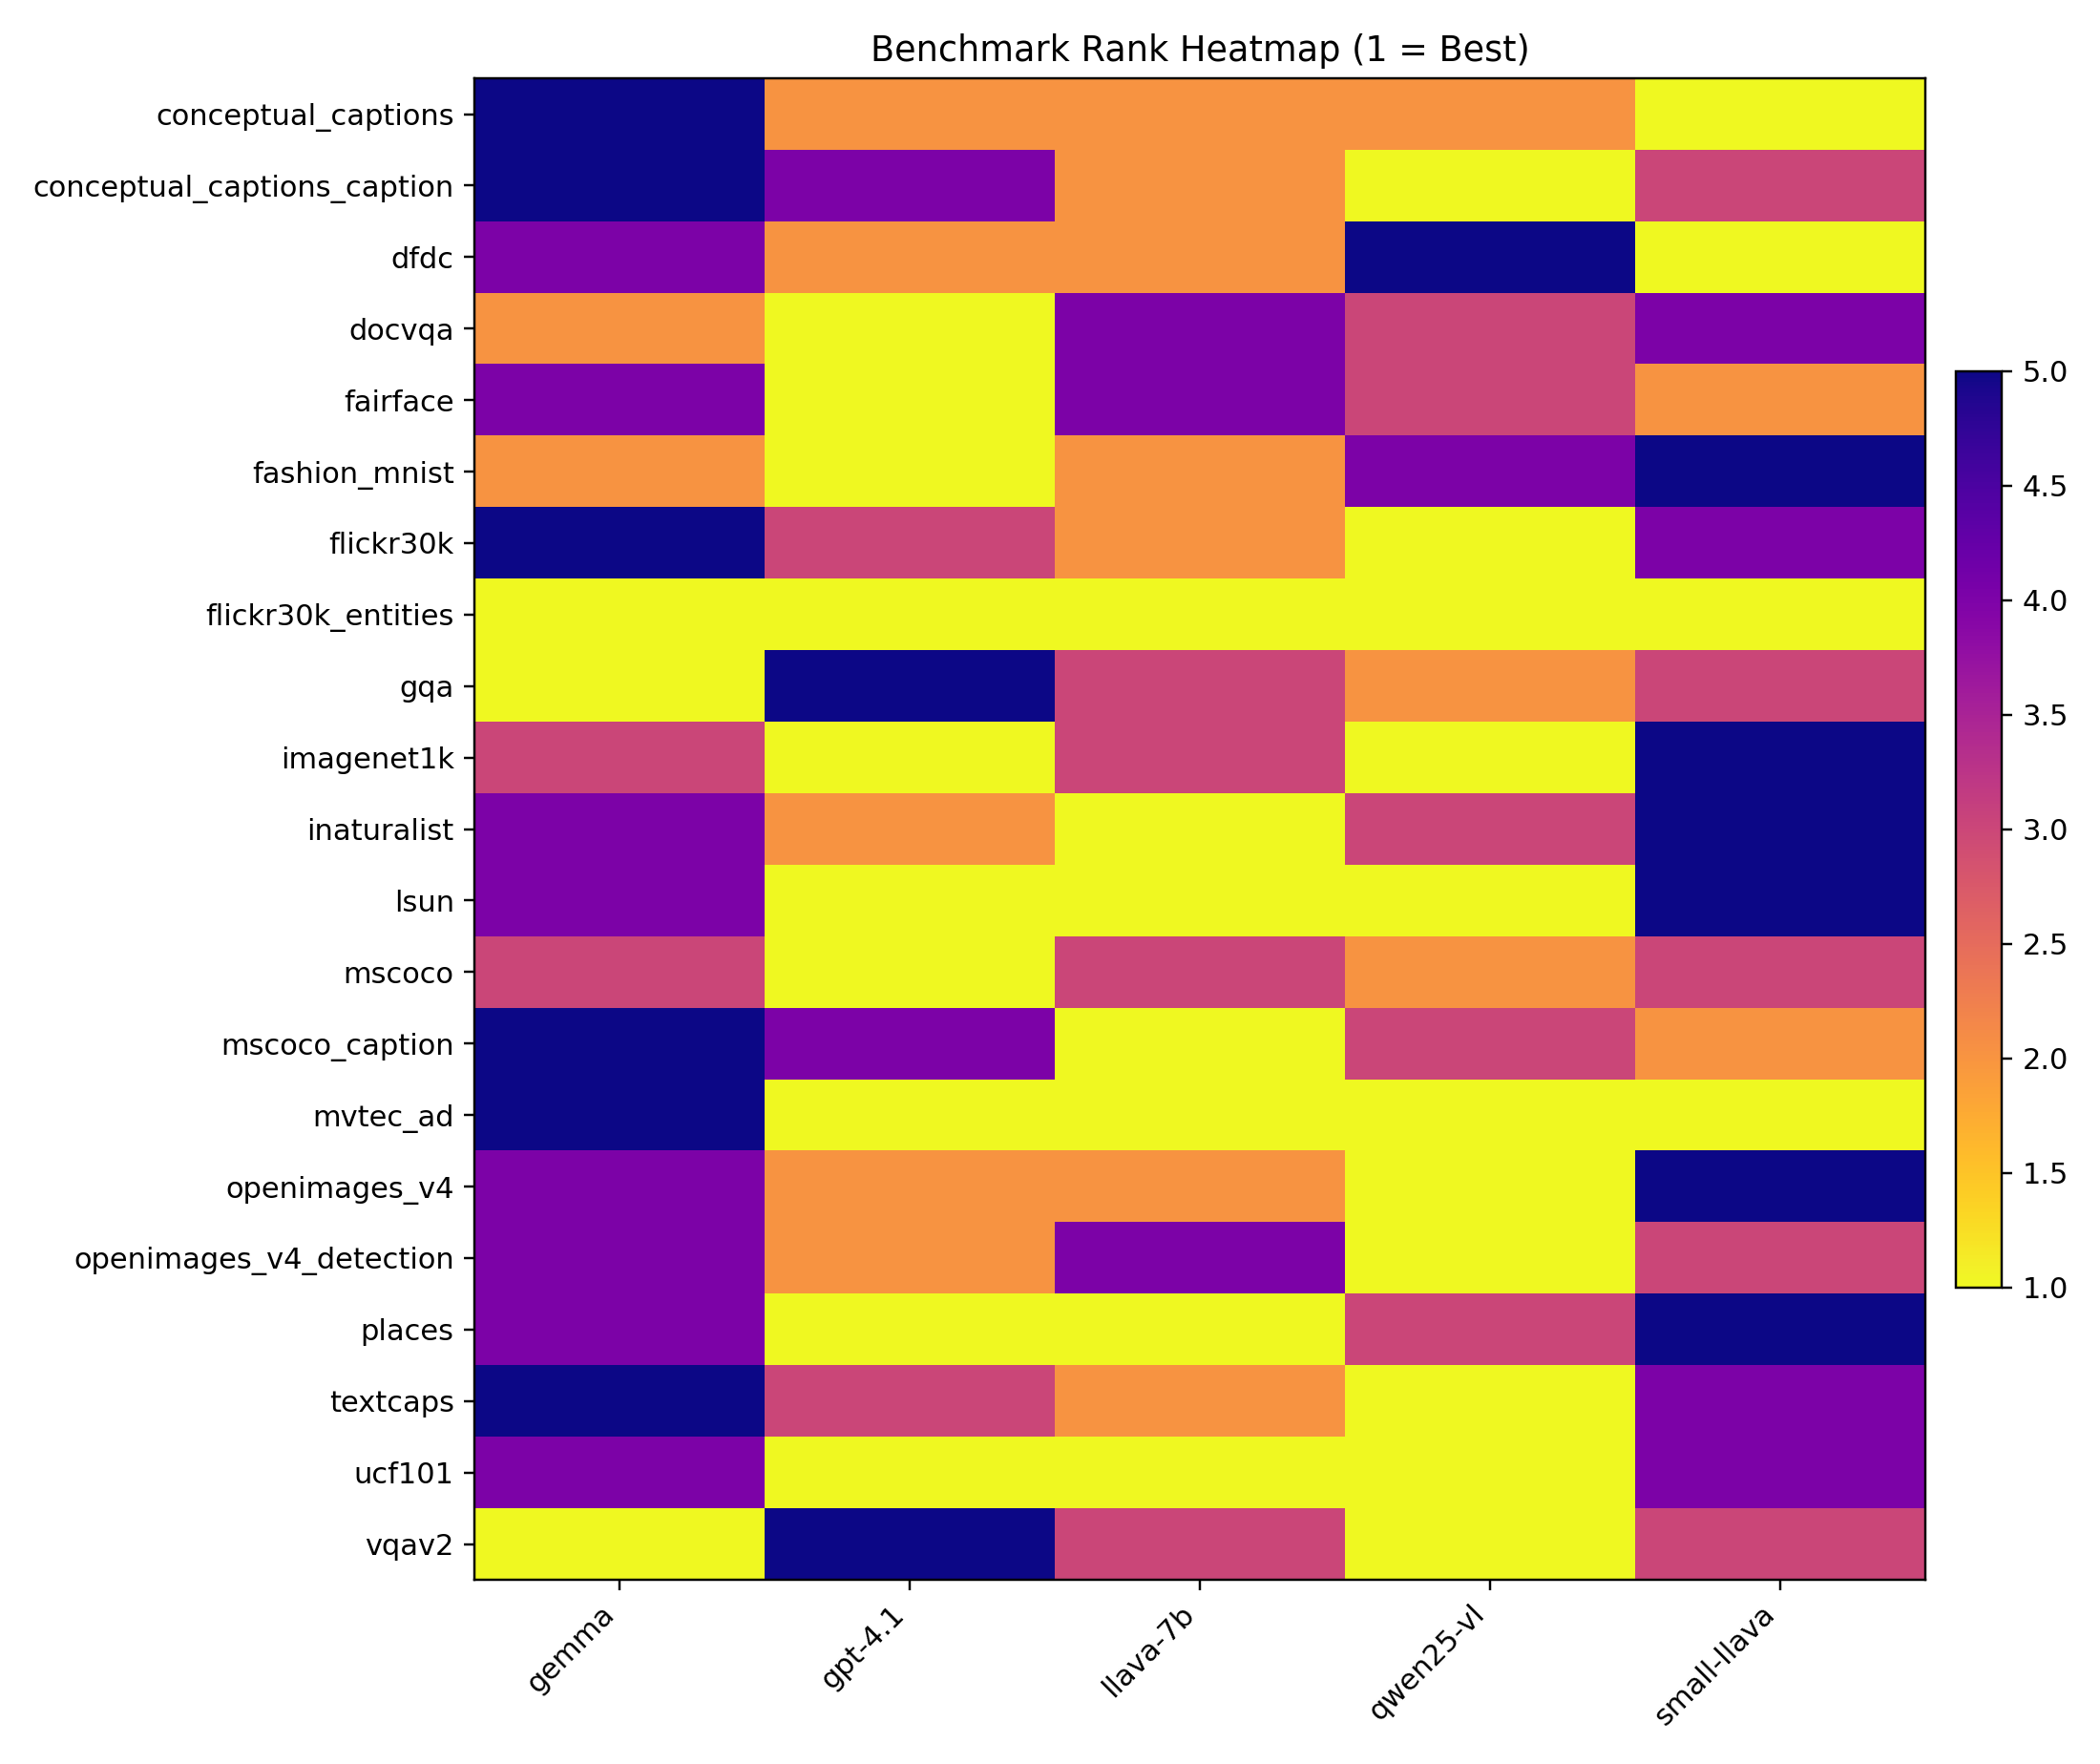
\includegraphics[width=\textwidth]{comparison/output/rank_heatmap.png}
\caption{Benchmark rank heatmap.}
\end{figure}

\begin{figure}[p]
\centering
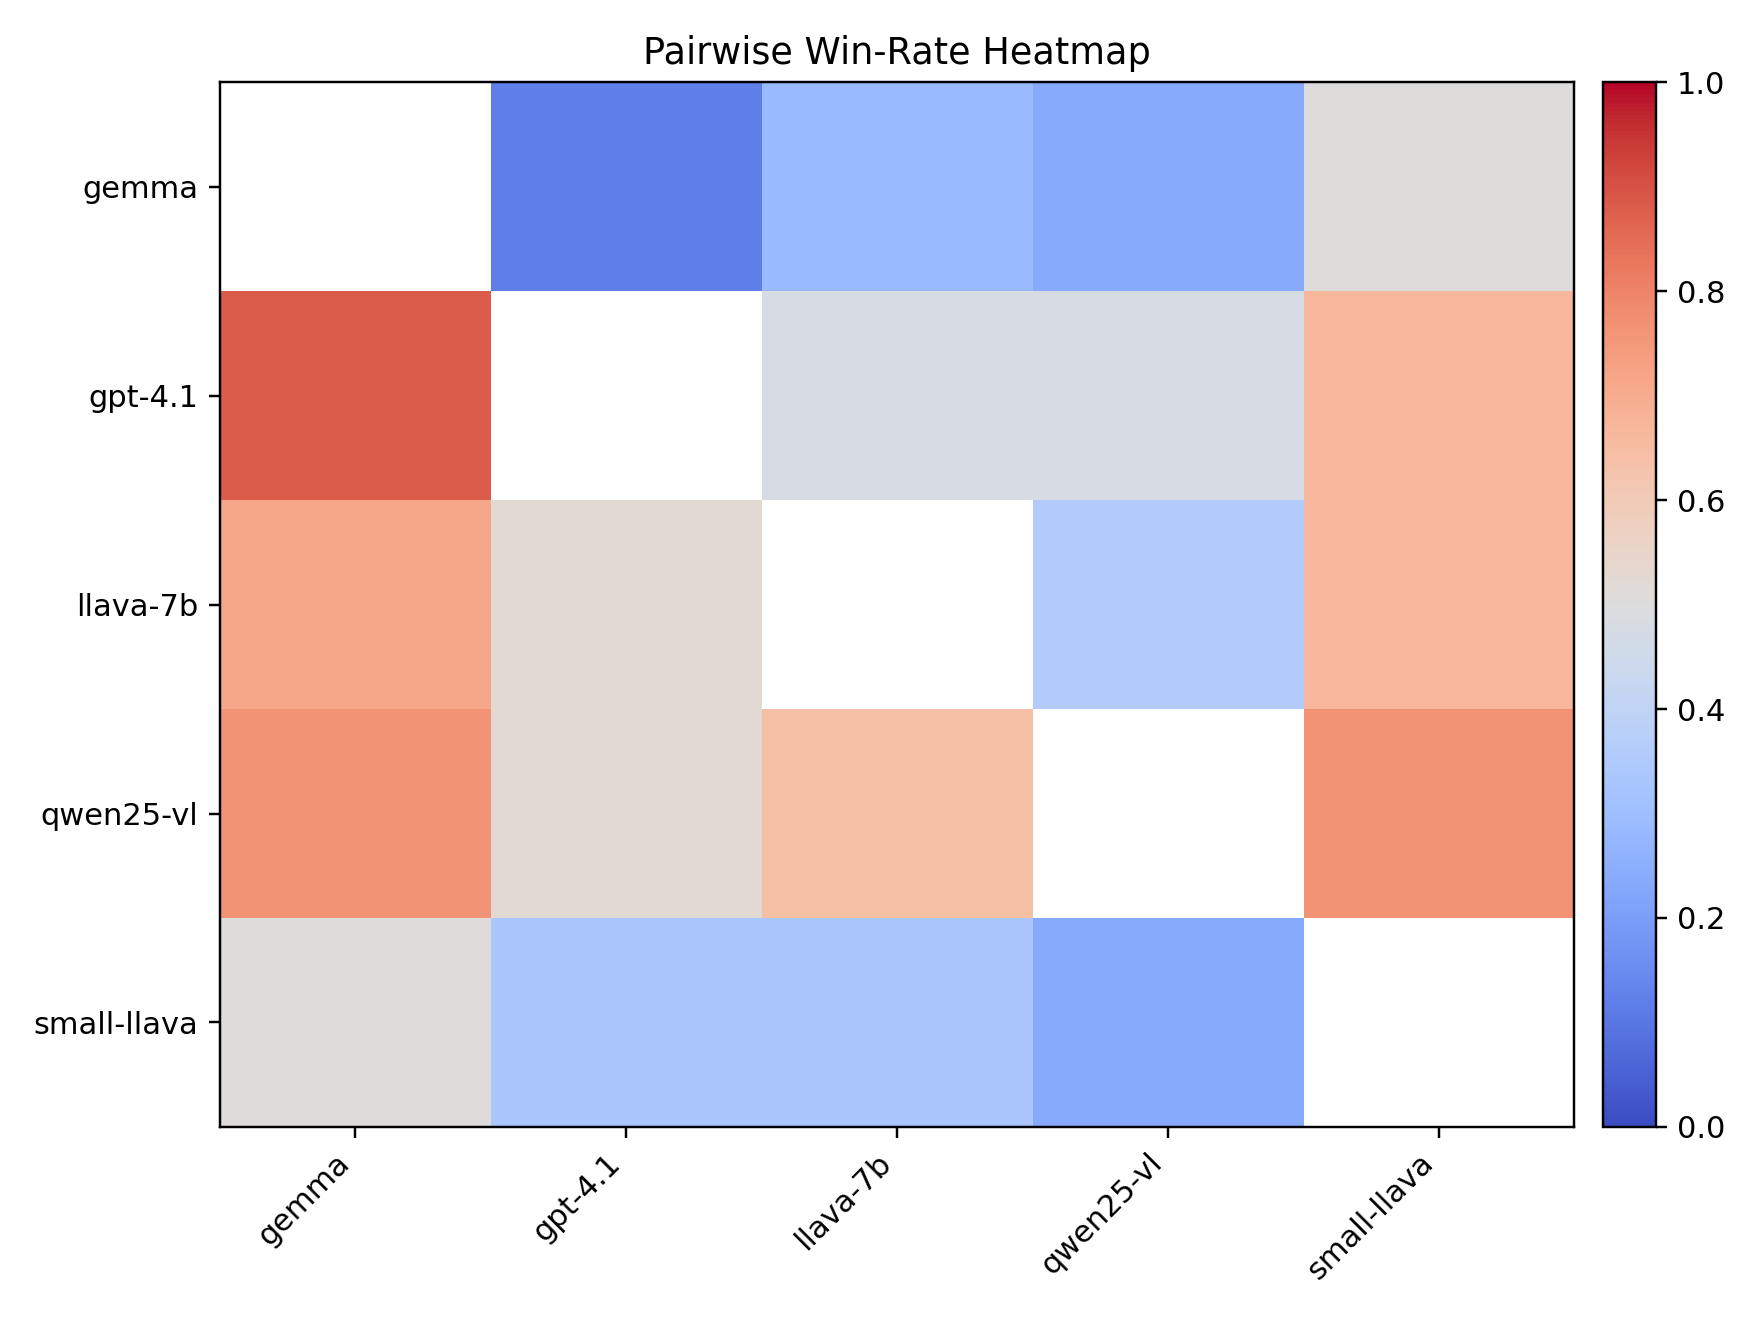
\includegraphics[width=\textwidth]{comparison/output/pairwise_win_rate_heatmap.png}
\caption{Pairwise win-rate heatmap.}
\end{figure}

\begin{figure}[p]
\centering
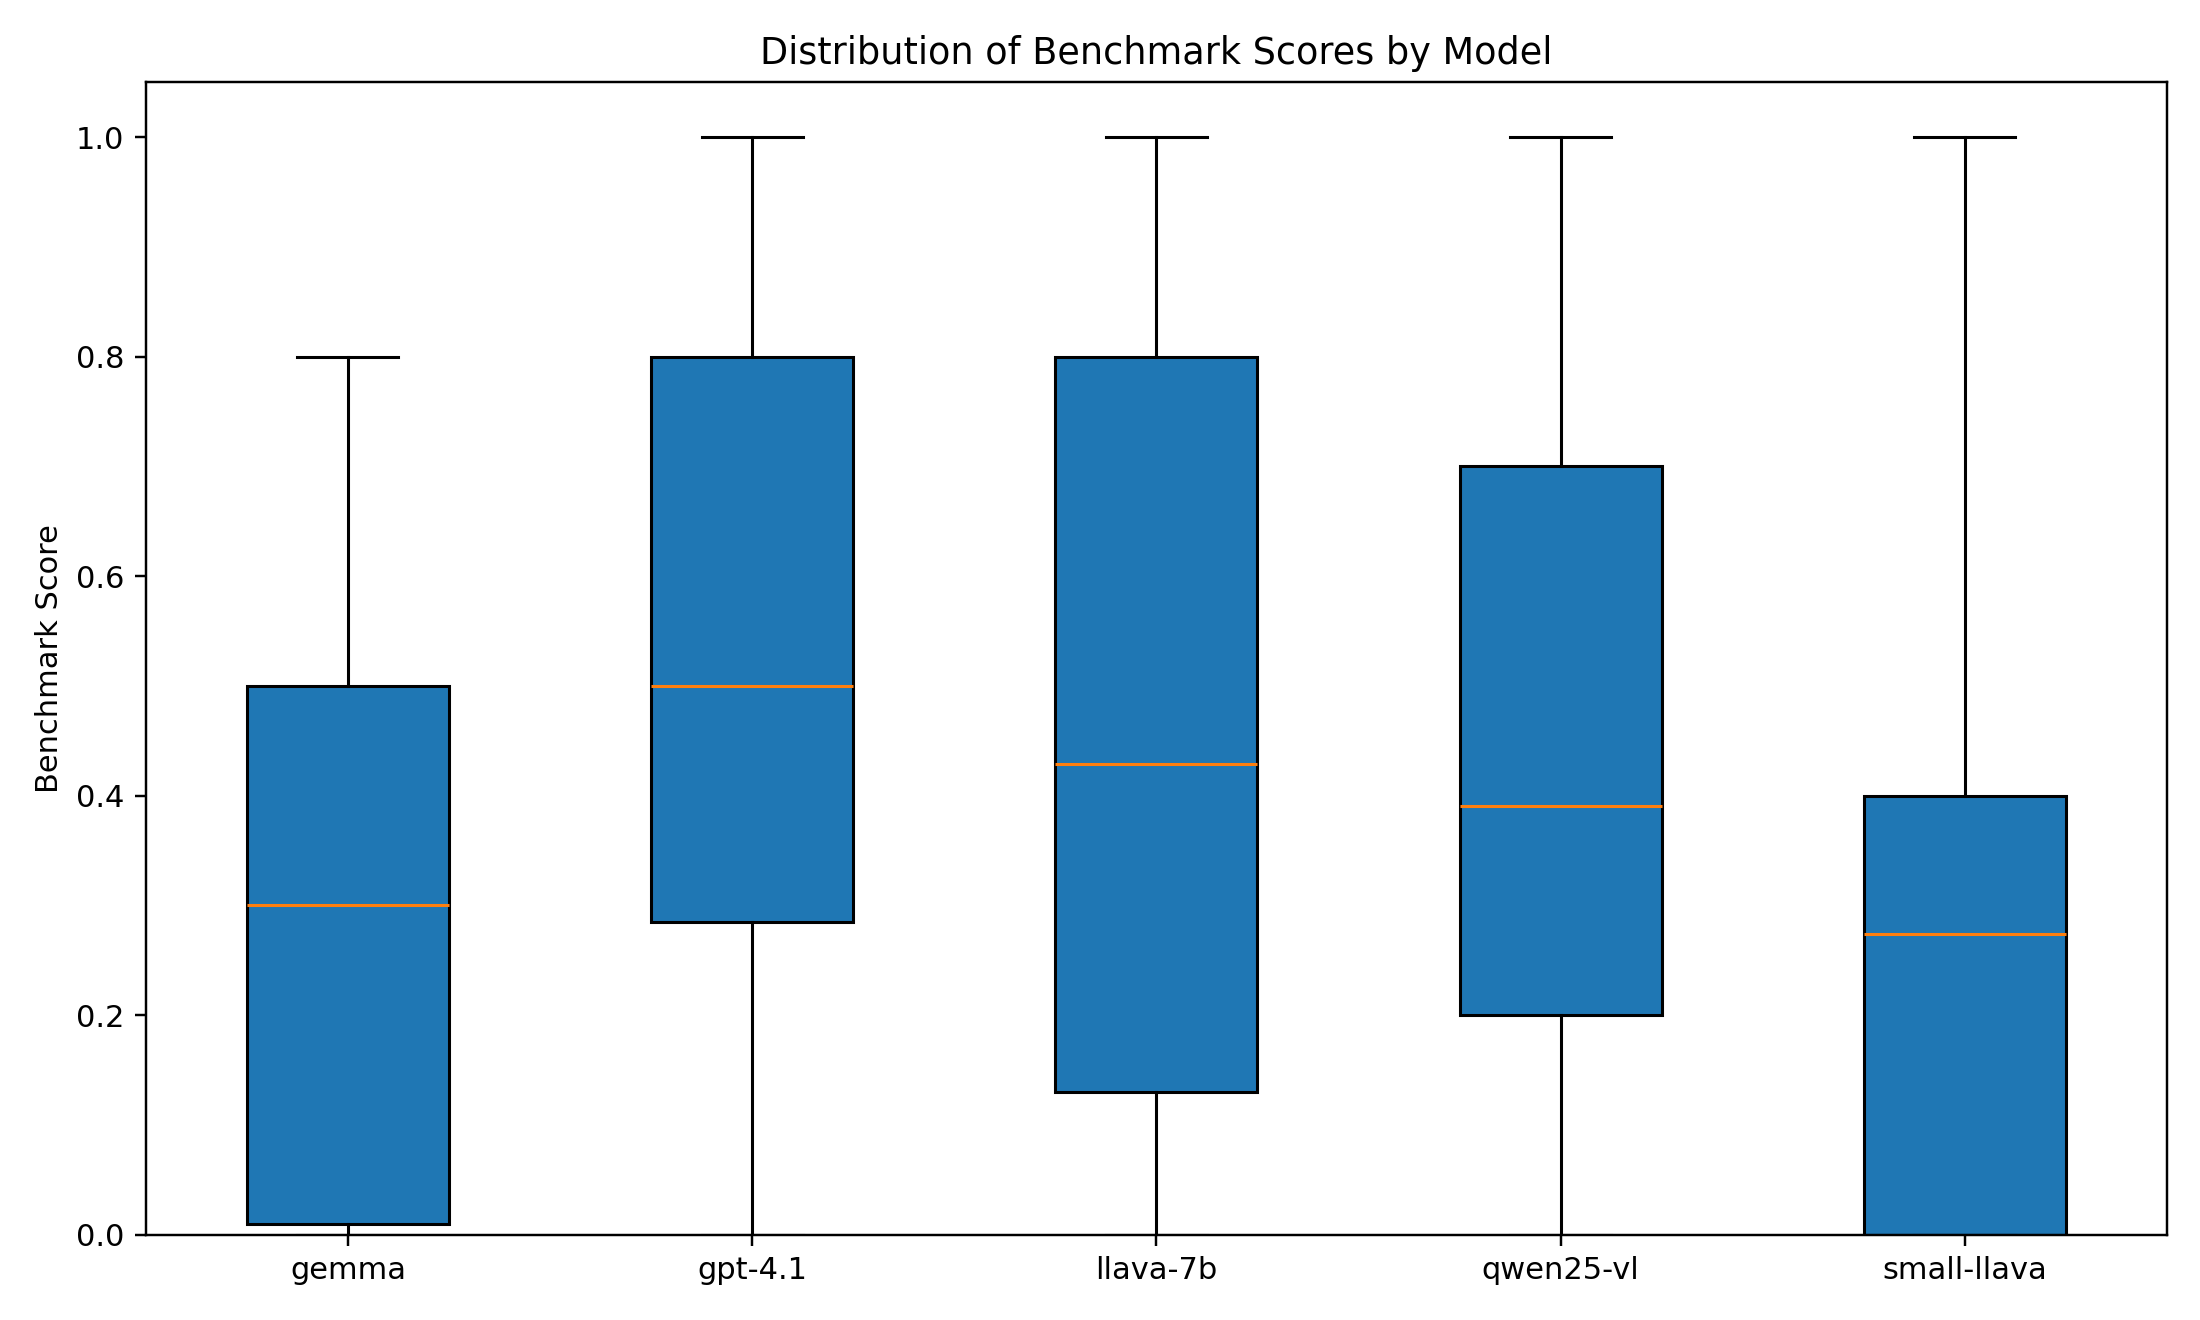
\includegraphics[width=\textwidth]{comparison/output/score_distribution_boxplot.png}
\caption{Score distribution boxplot.}
\end{figure}

\begin{figure}[p]
\centering
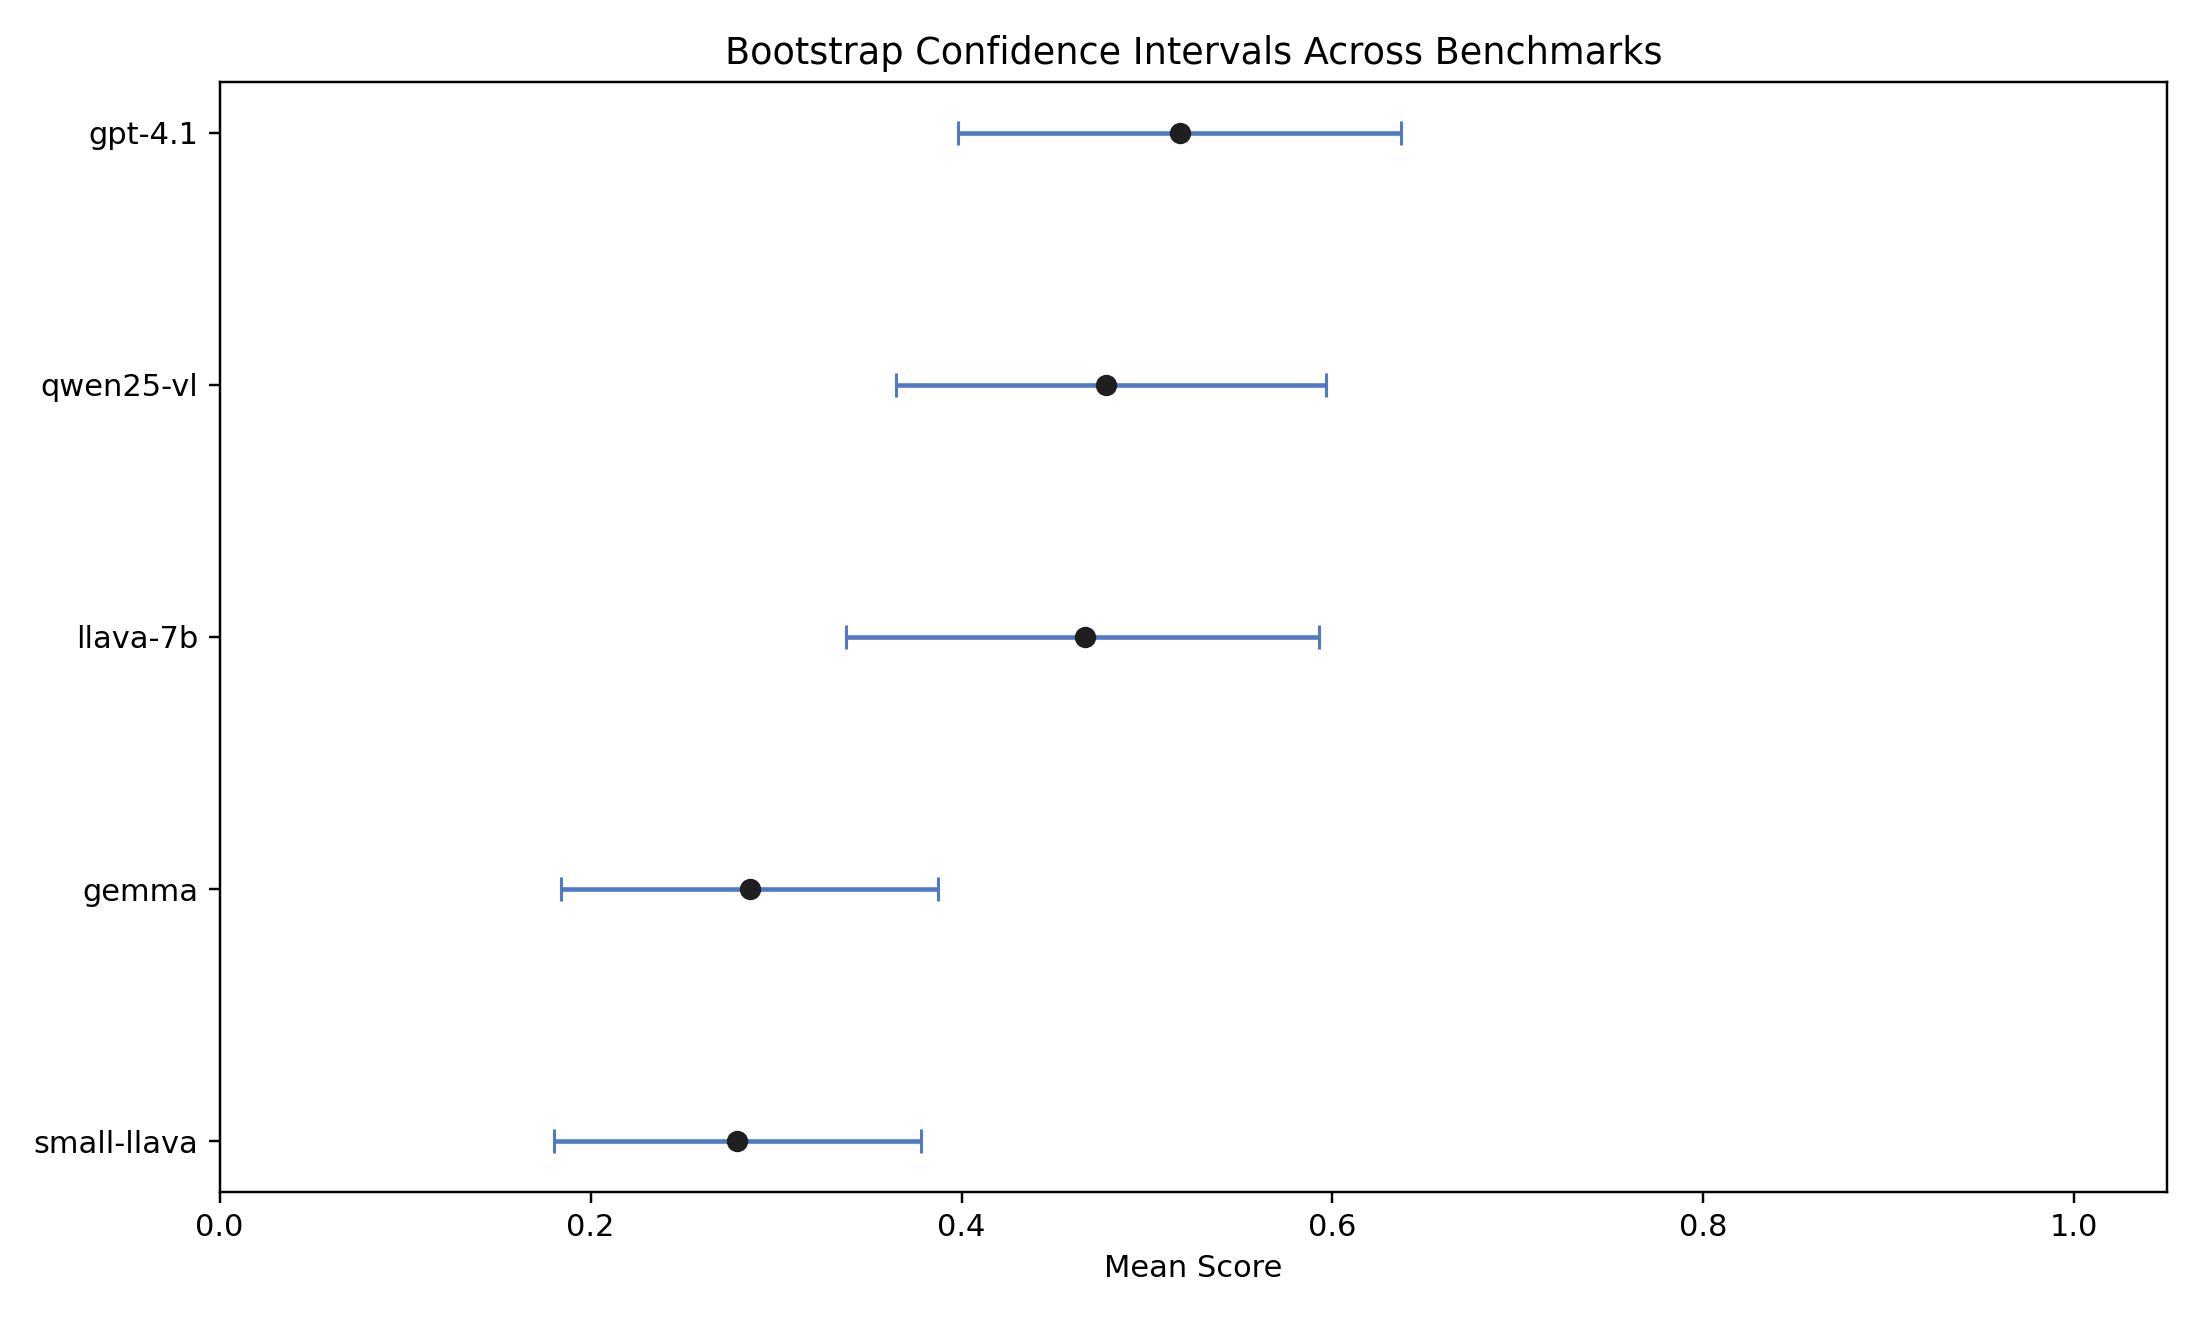
\includegraphics[width=\textwidth]{comparison/output/bootstrap_confidence_intervals.png}
\caption{Bootstrap confidence intervals over benchmarks.}
\end{figure}

\begin{figure}[p]
\centering
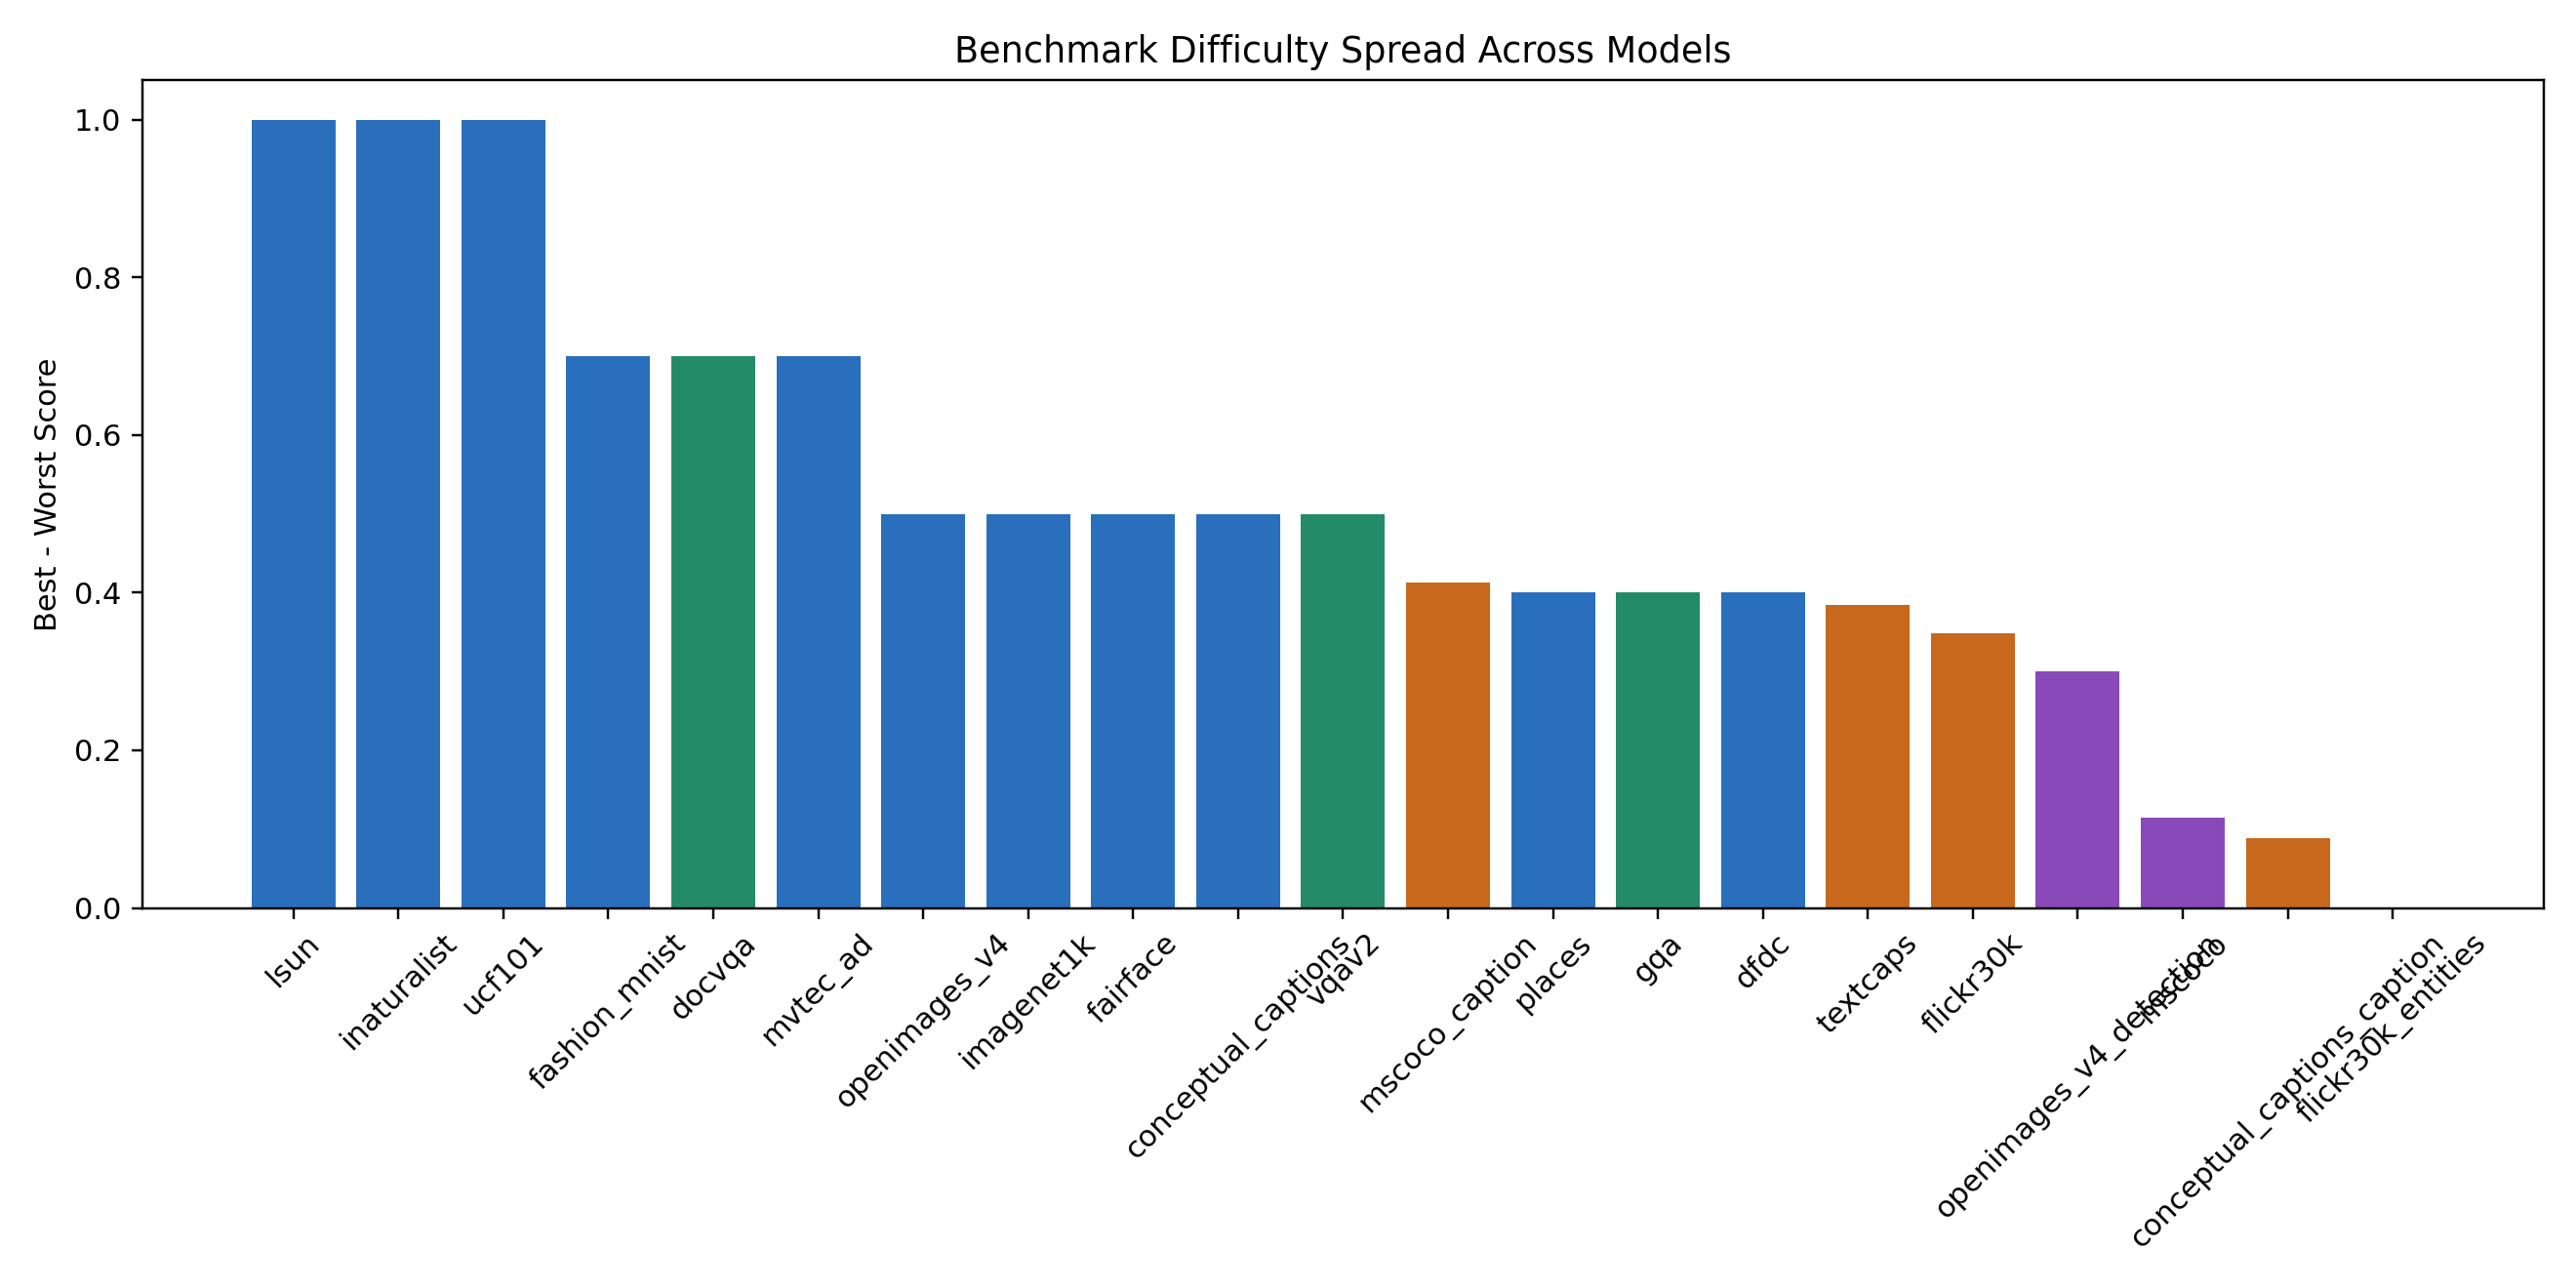
\includegraphics[width=\textwidth]{comparison/output/benchmark_spread.png}
\caption{Benchmark spread across models.}
\end{figure}

\begin{figure}[p]
\centering
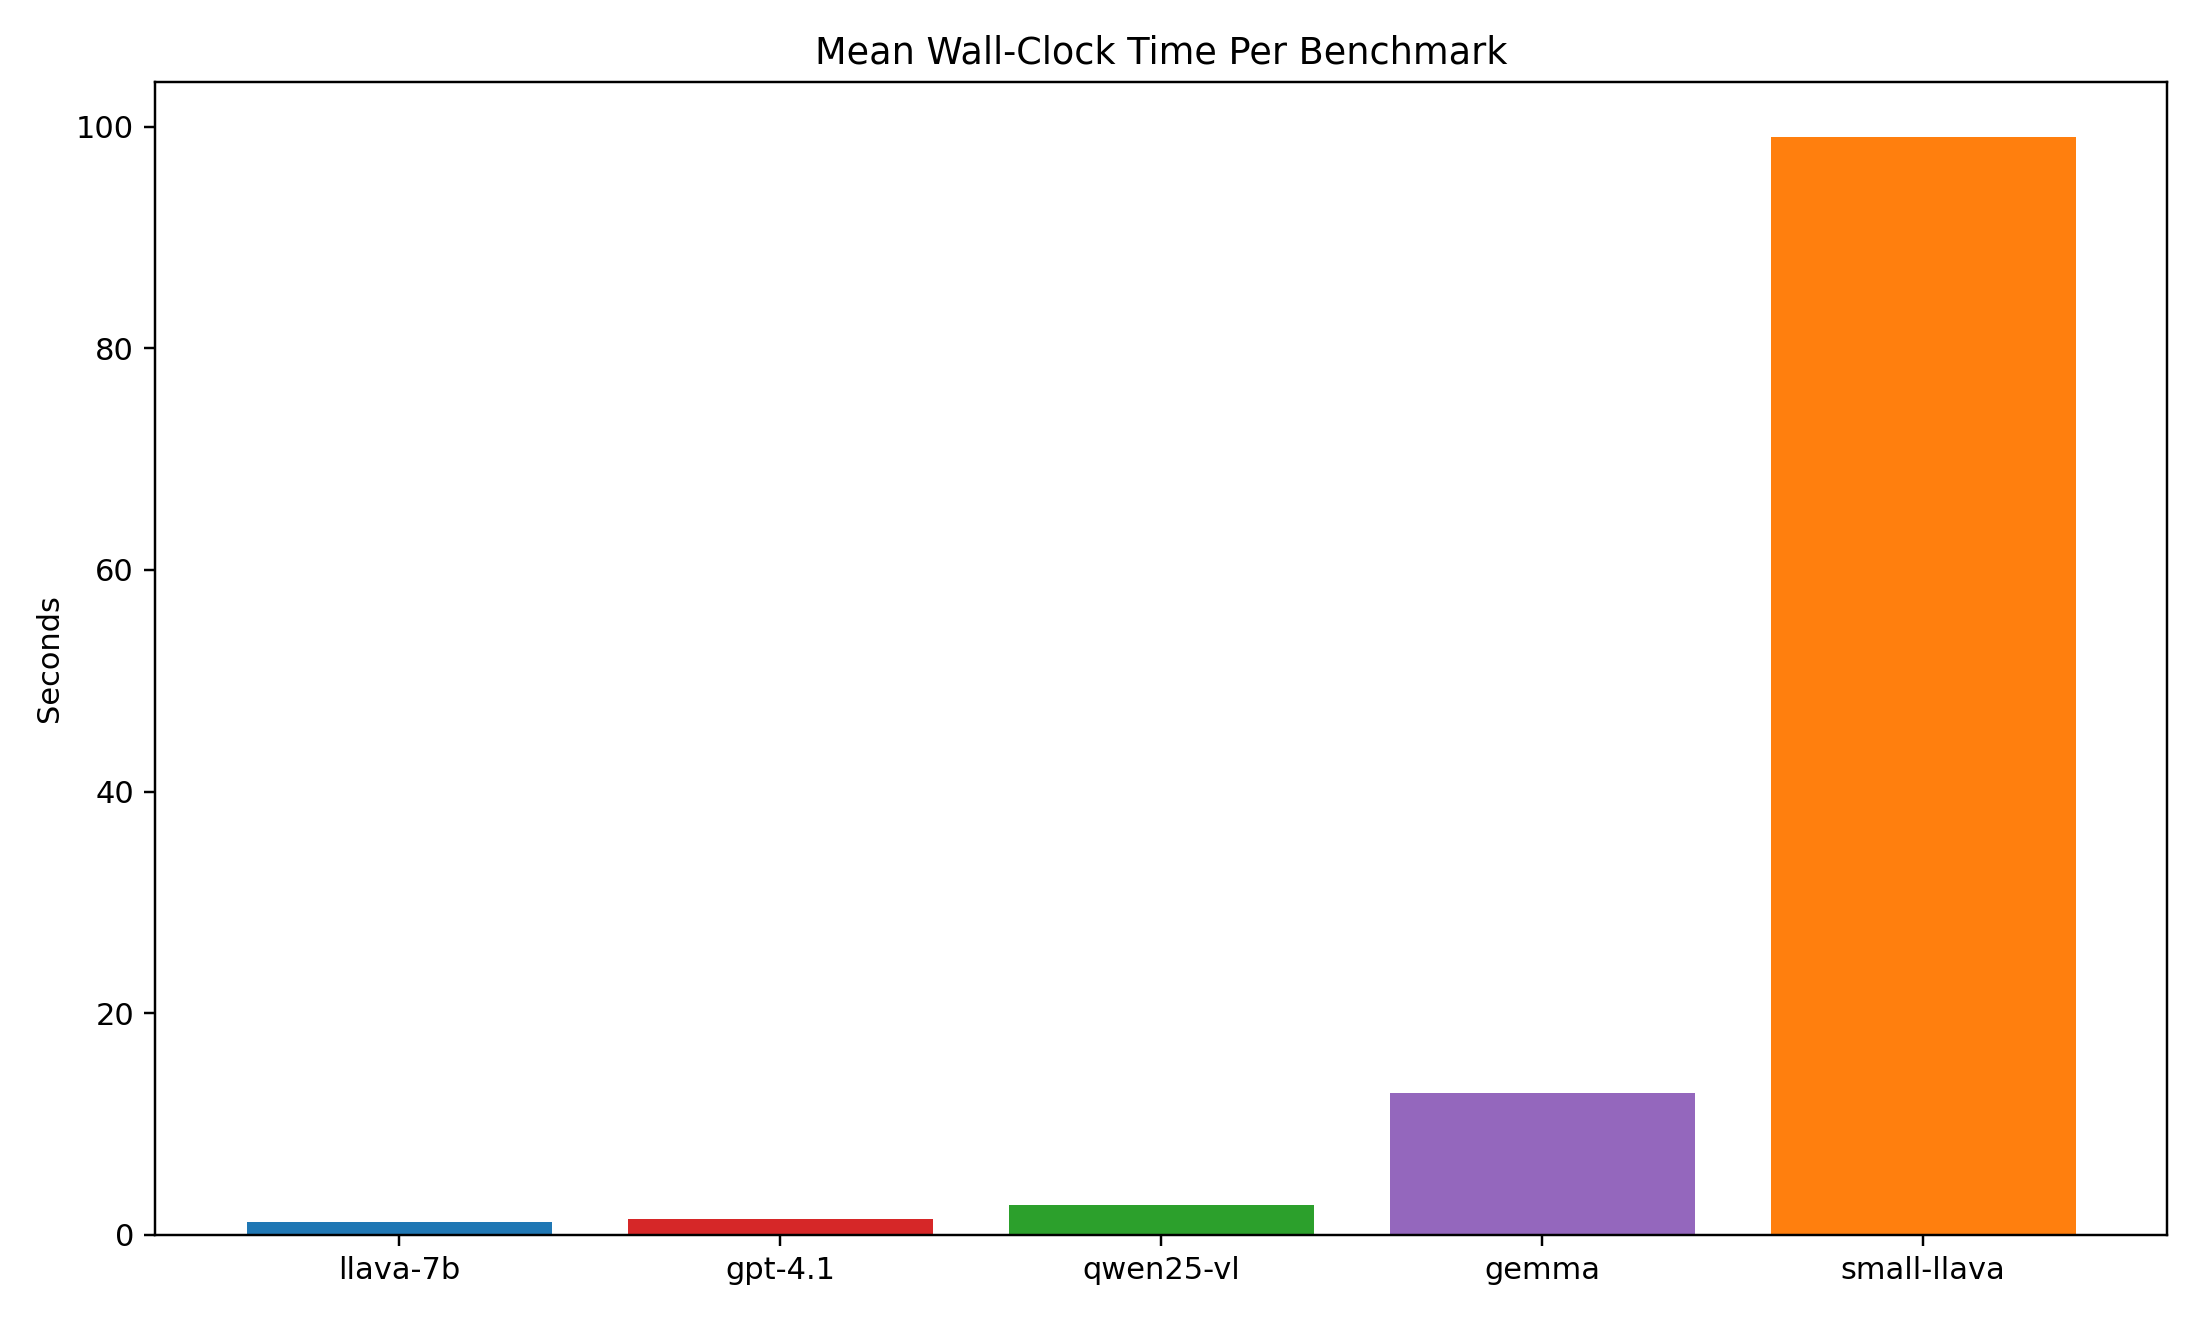
\includegraphics[width=\textwidth]{comparison/output/telemetry_mean_wall_clock_seconds.png}
\caption{Mean wall-clock time by model.}
\end{figure}

\begin{figure}[p]
\centering
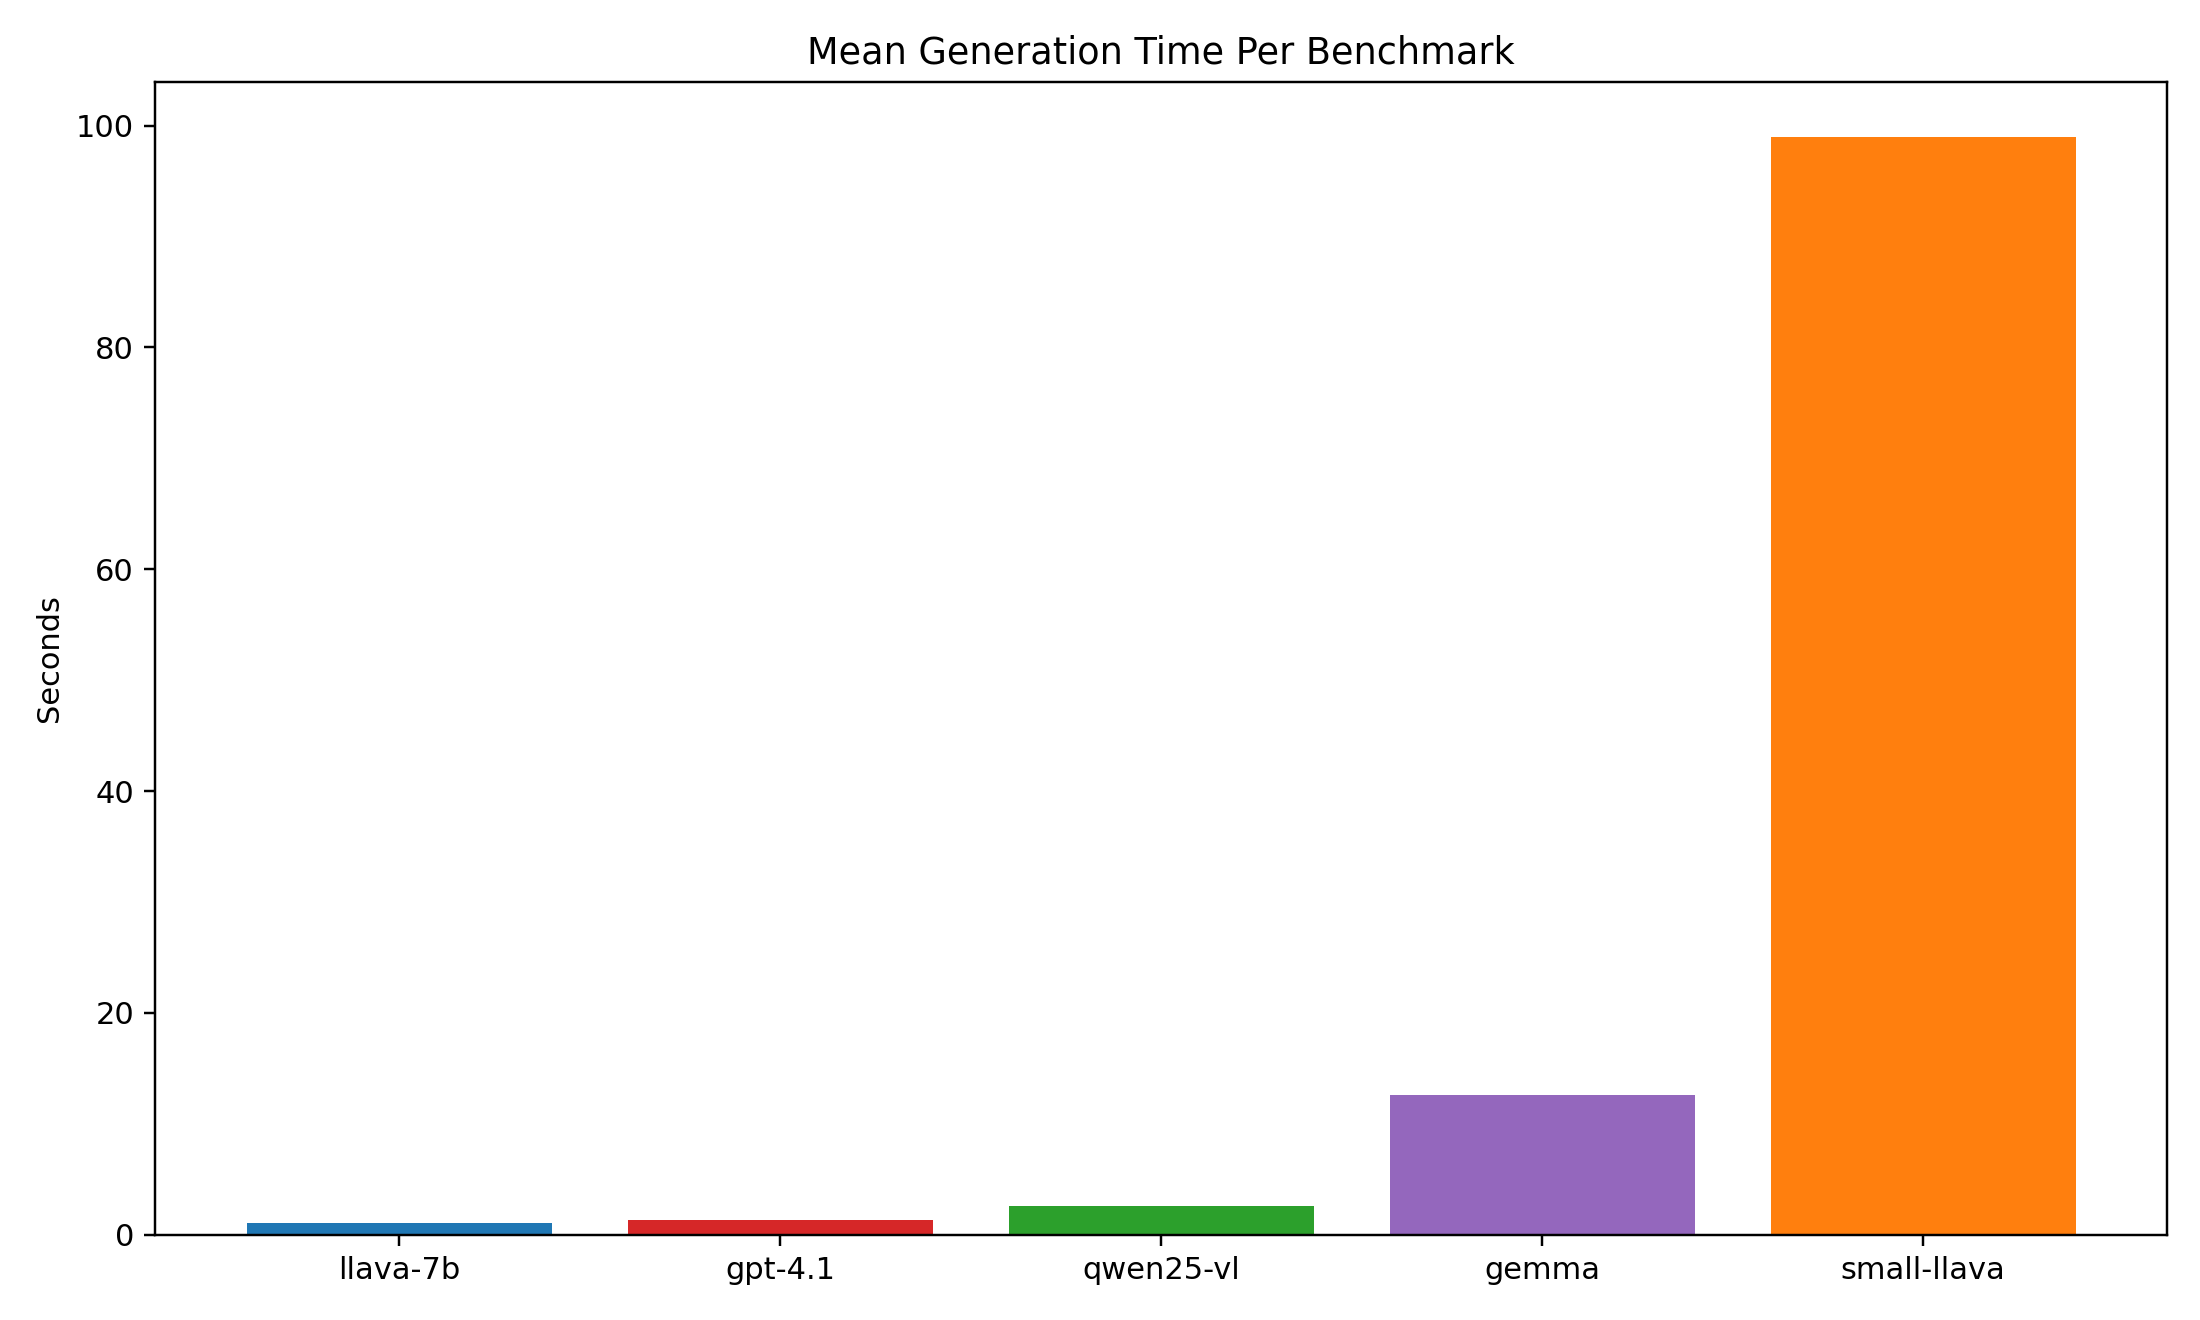
\includegraphics[width=\textwidth]{comparison/output/telemetry_mean_generation_seconds.png}
\caption{Mean generation time by model.}
\end{figure}

\begin{figure}[p]
\centering
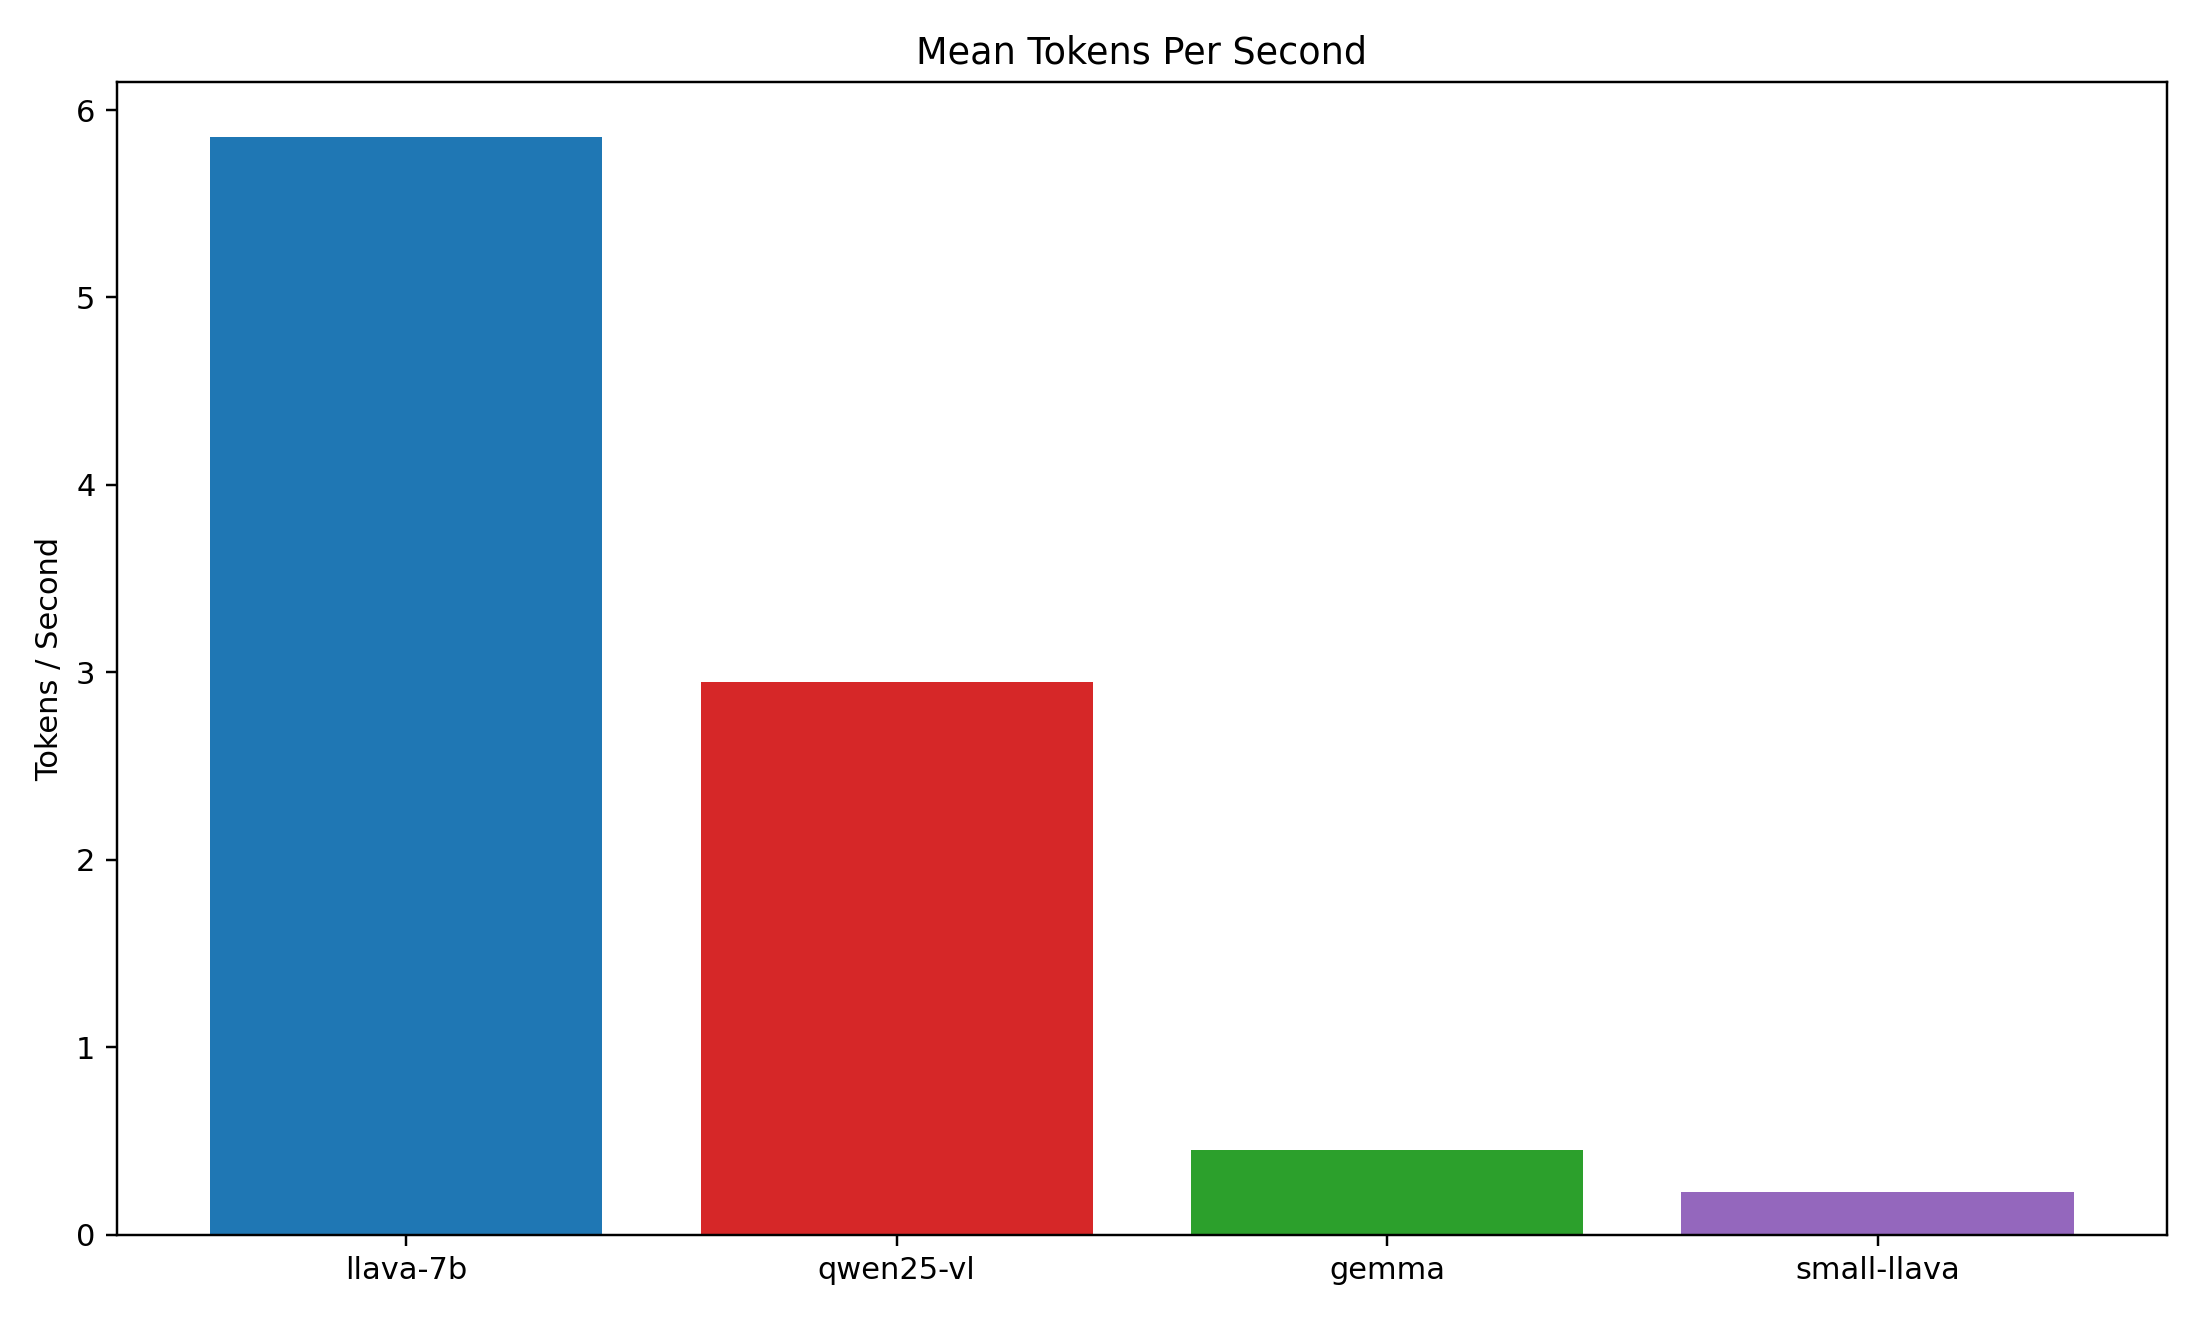
\includegraphics[width=\textwidth]{comparison/output/telemetry_mean_tokens_per_second.png}
\caption{Mean tokens per second by model.}
\end{figure}

\begin{figure}[p]
\centering
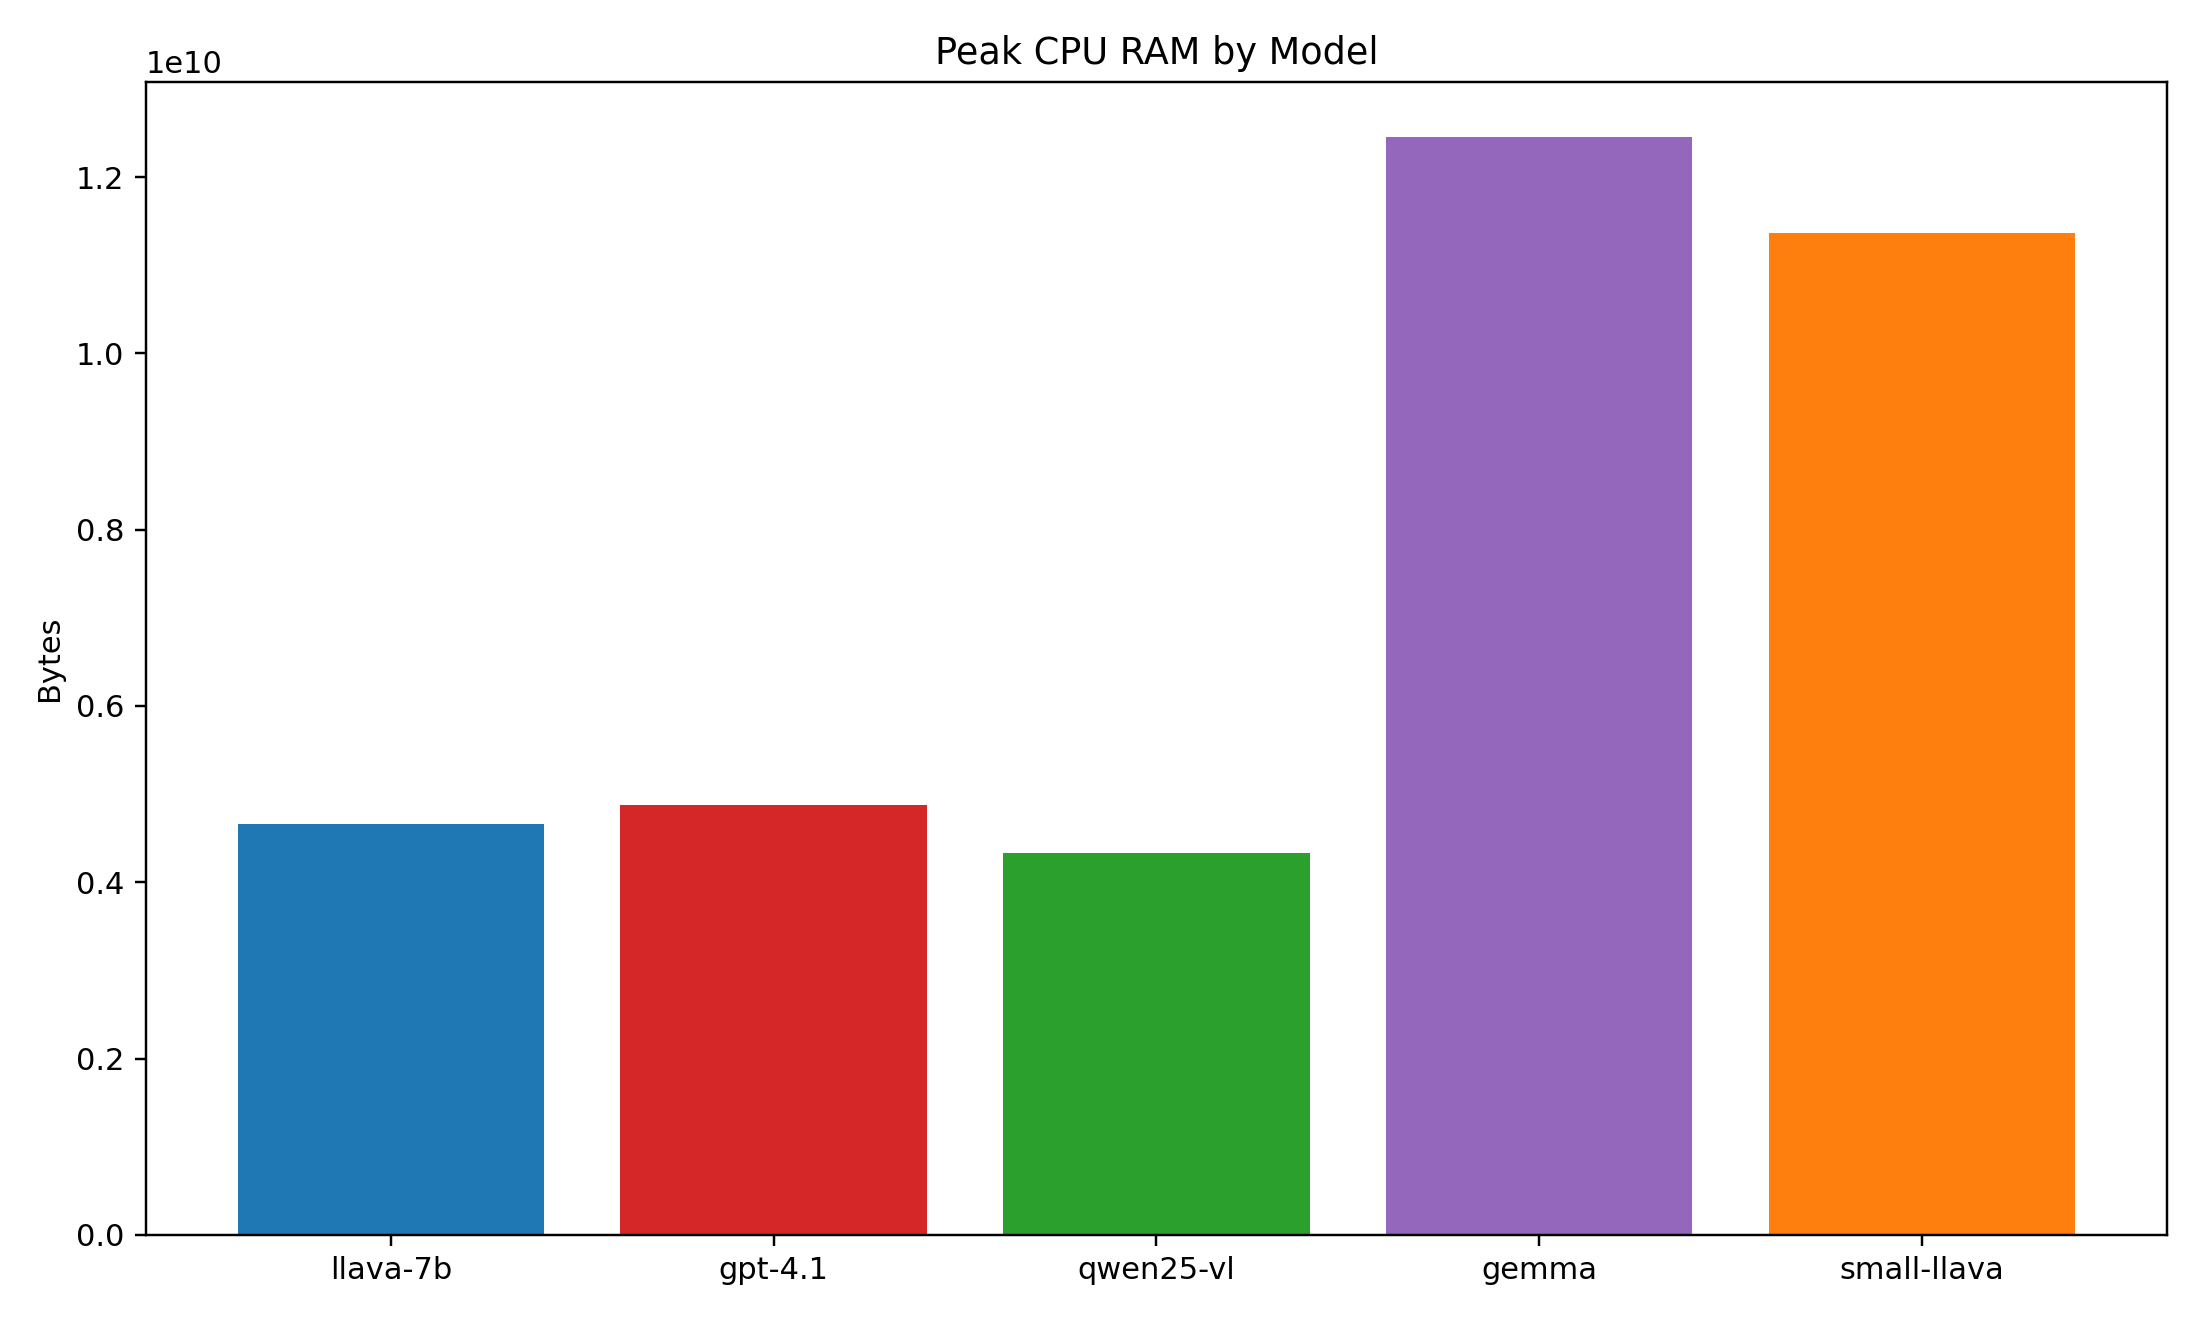
\includegraphics[width=\textwidth]{comparison/output/telemetry_peak_cpu_ram_gib.png}
\caption{Peak CPU RAM usage by model.}
\end{figure}

\begin{figure}[p]
\centering
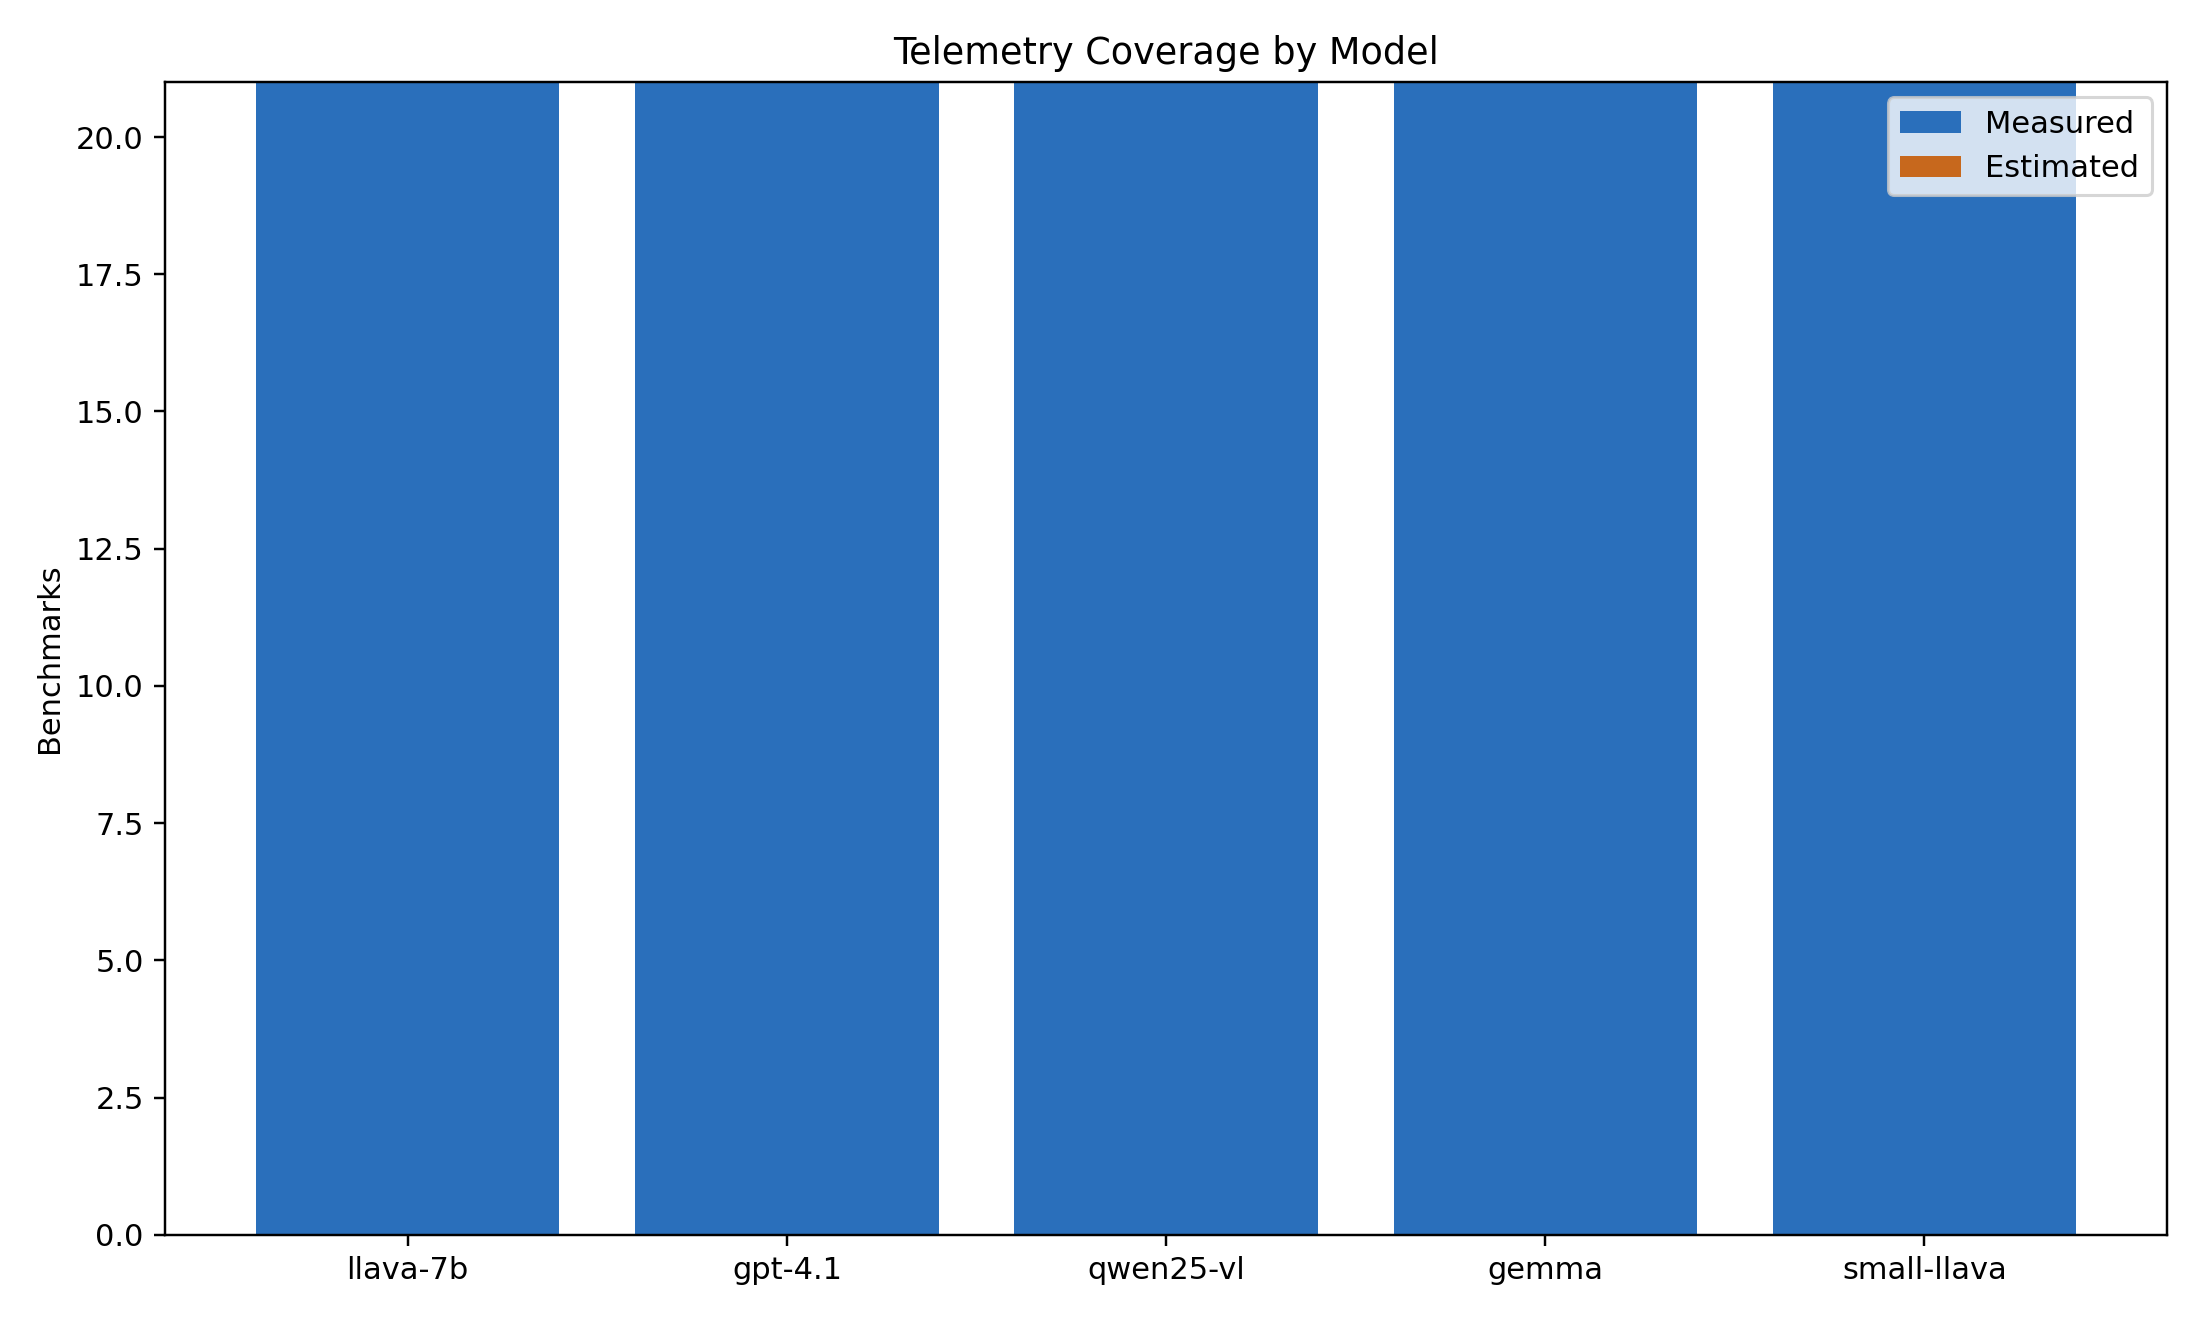
\includegraphics[width=\textwidth]{comparison/output/telemetry_coverage.png}
\caption{Telemetry coverage across saved benchmark results.}
\end{figure}

\begin{figure}[p]
\centering
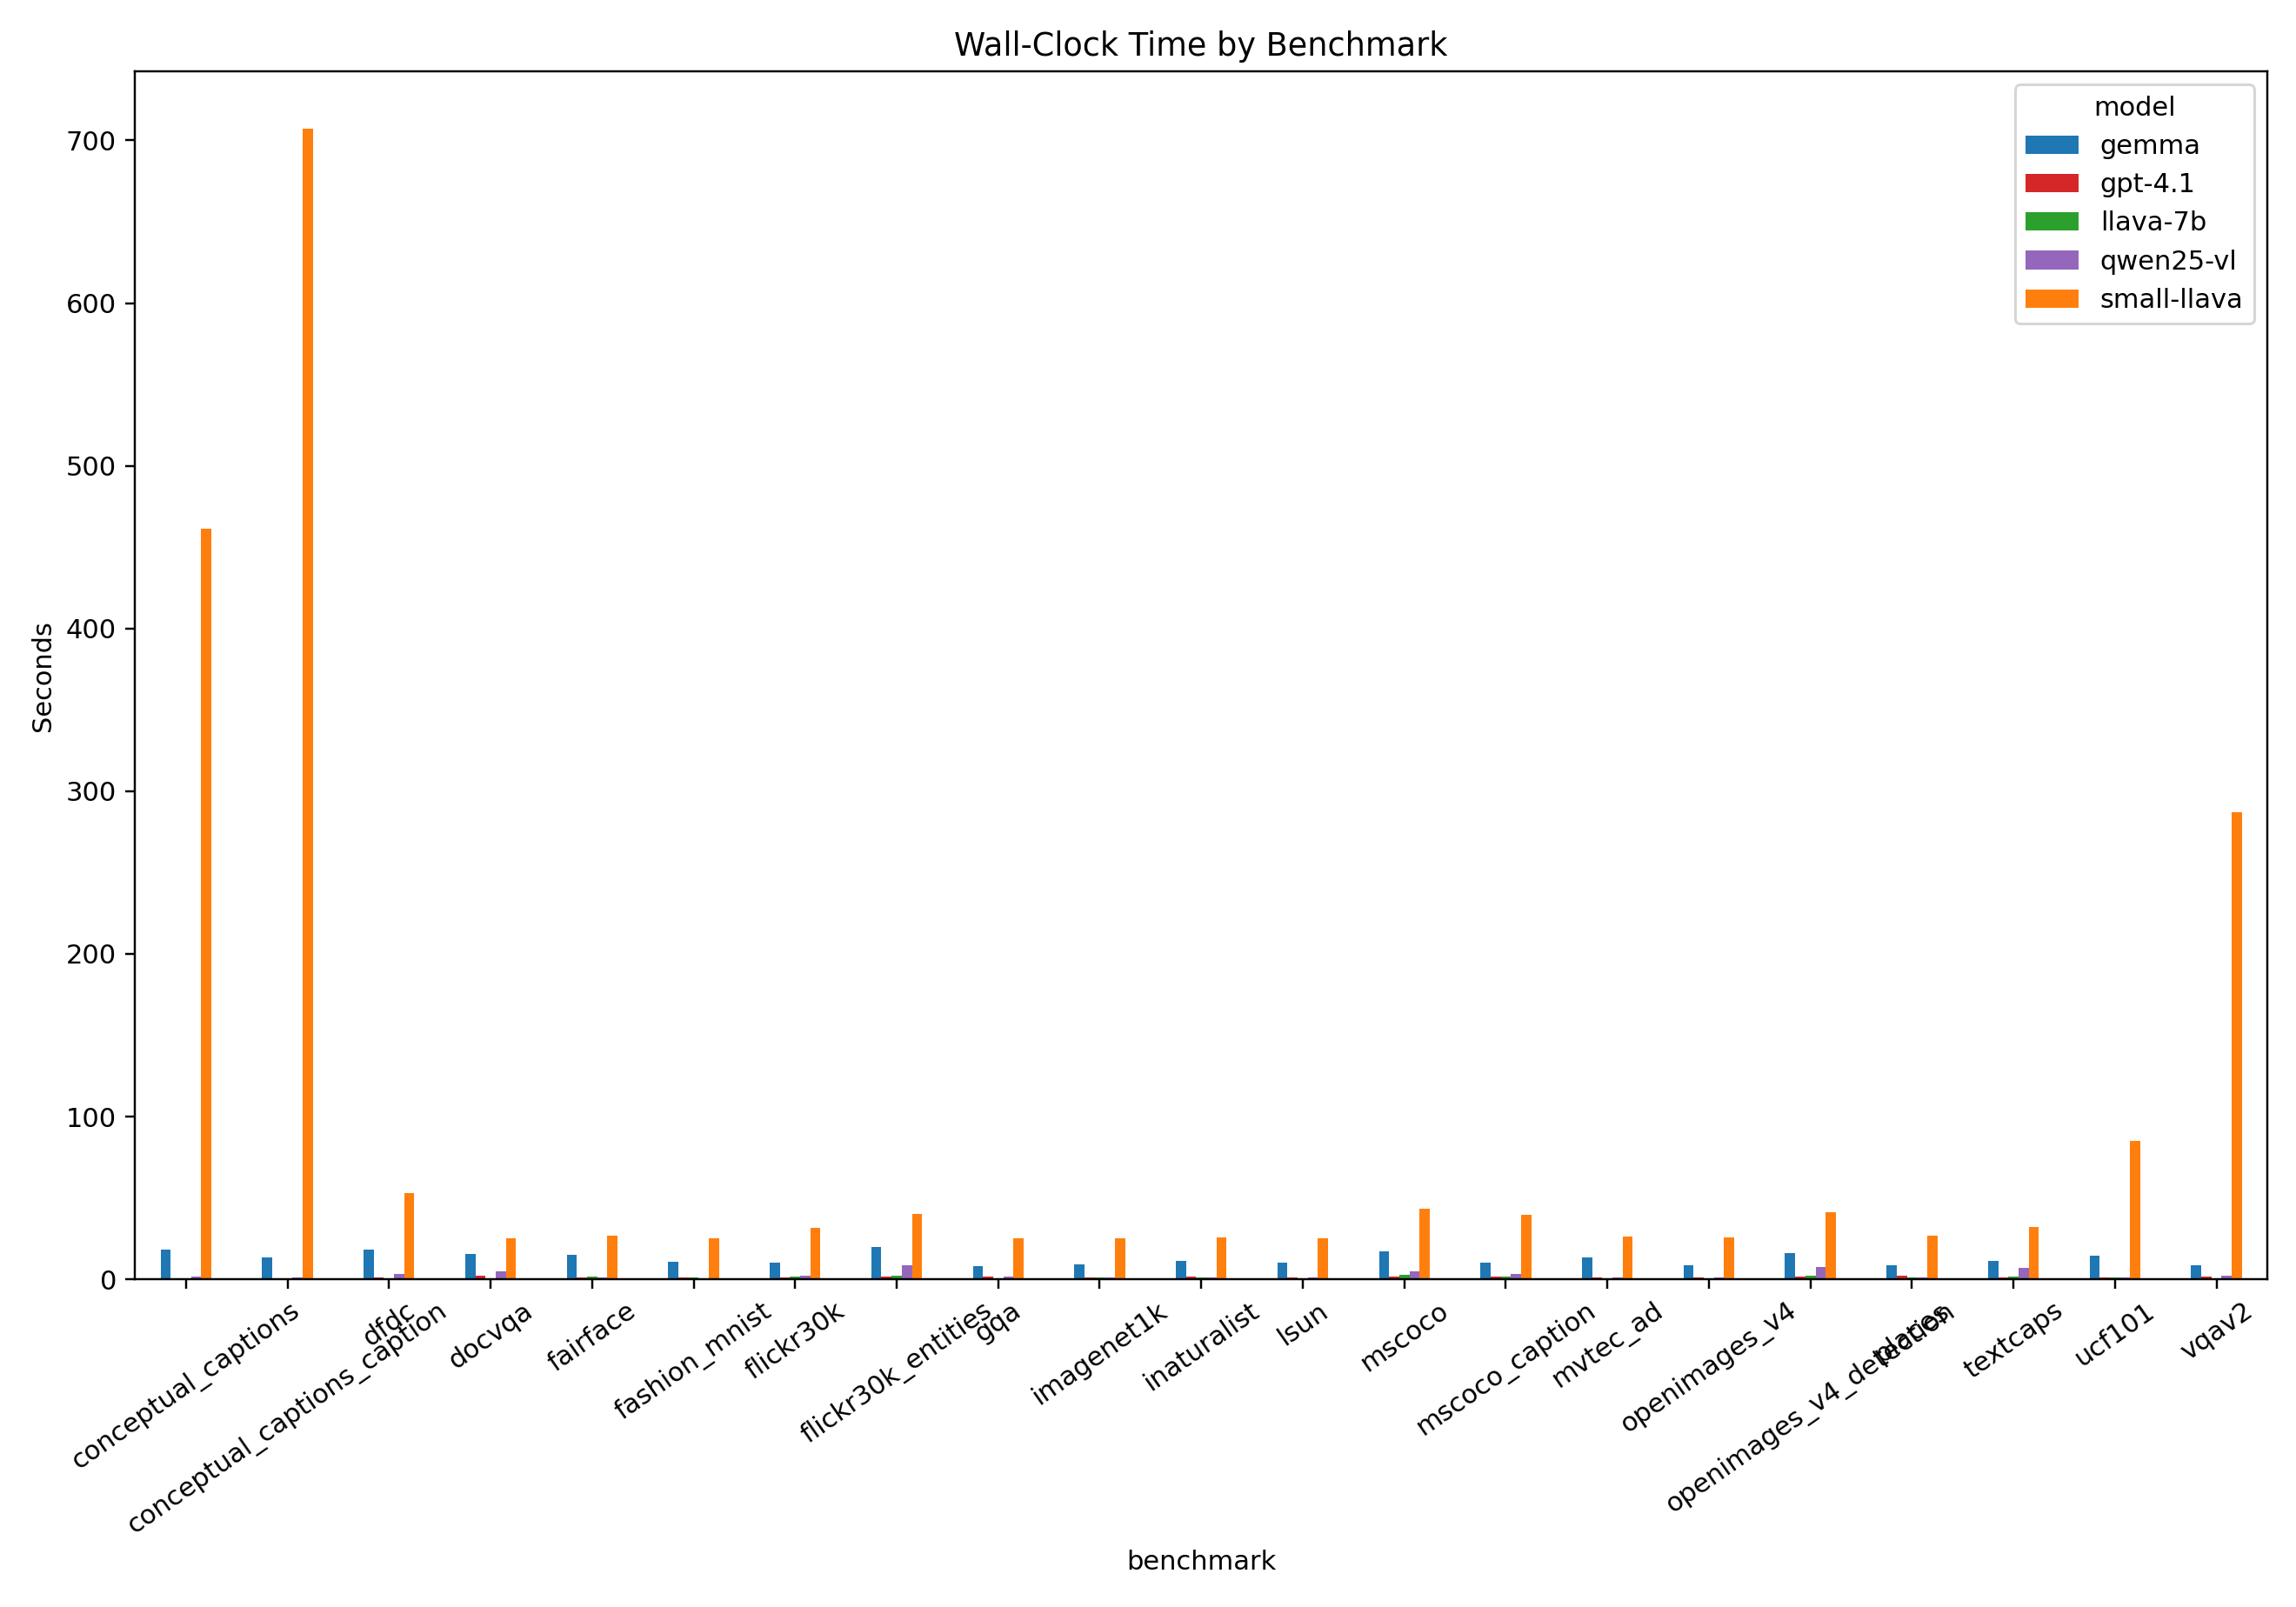
\includegraphics[width=\textwidth]{comparison/output/telemetry_wall_clock_by_benchmark.png}
\caption{Wall-clock time by benchmark.}
\end{figure}

\begin{figure}[p]
\centering
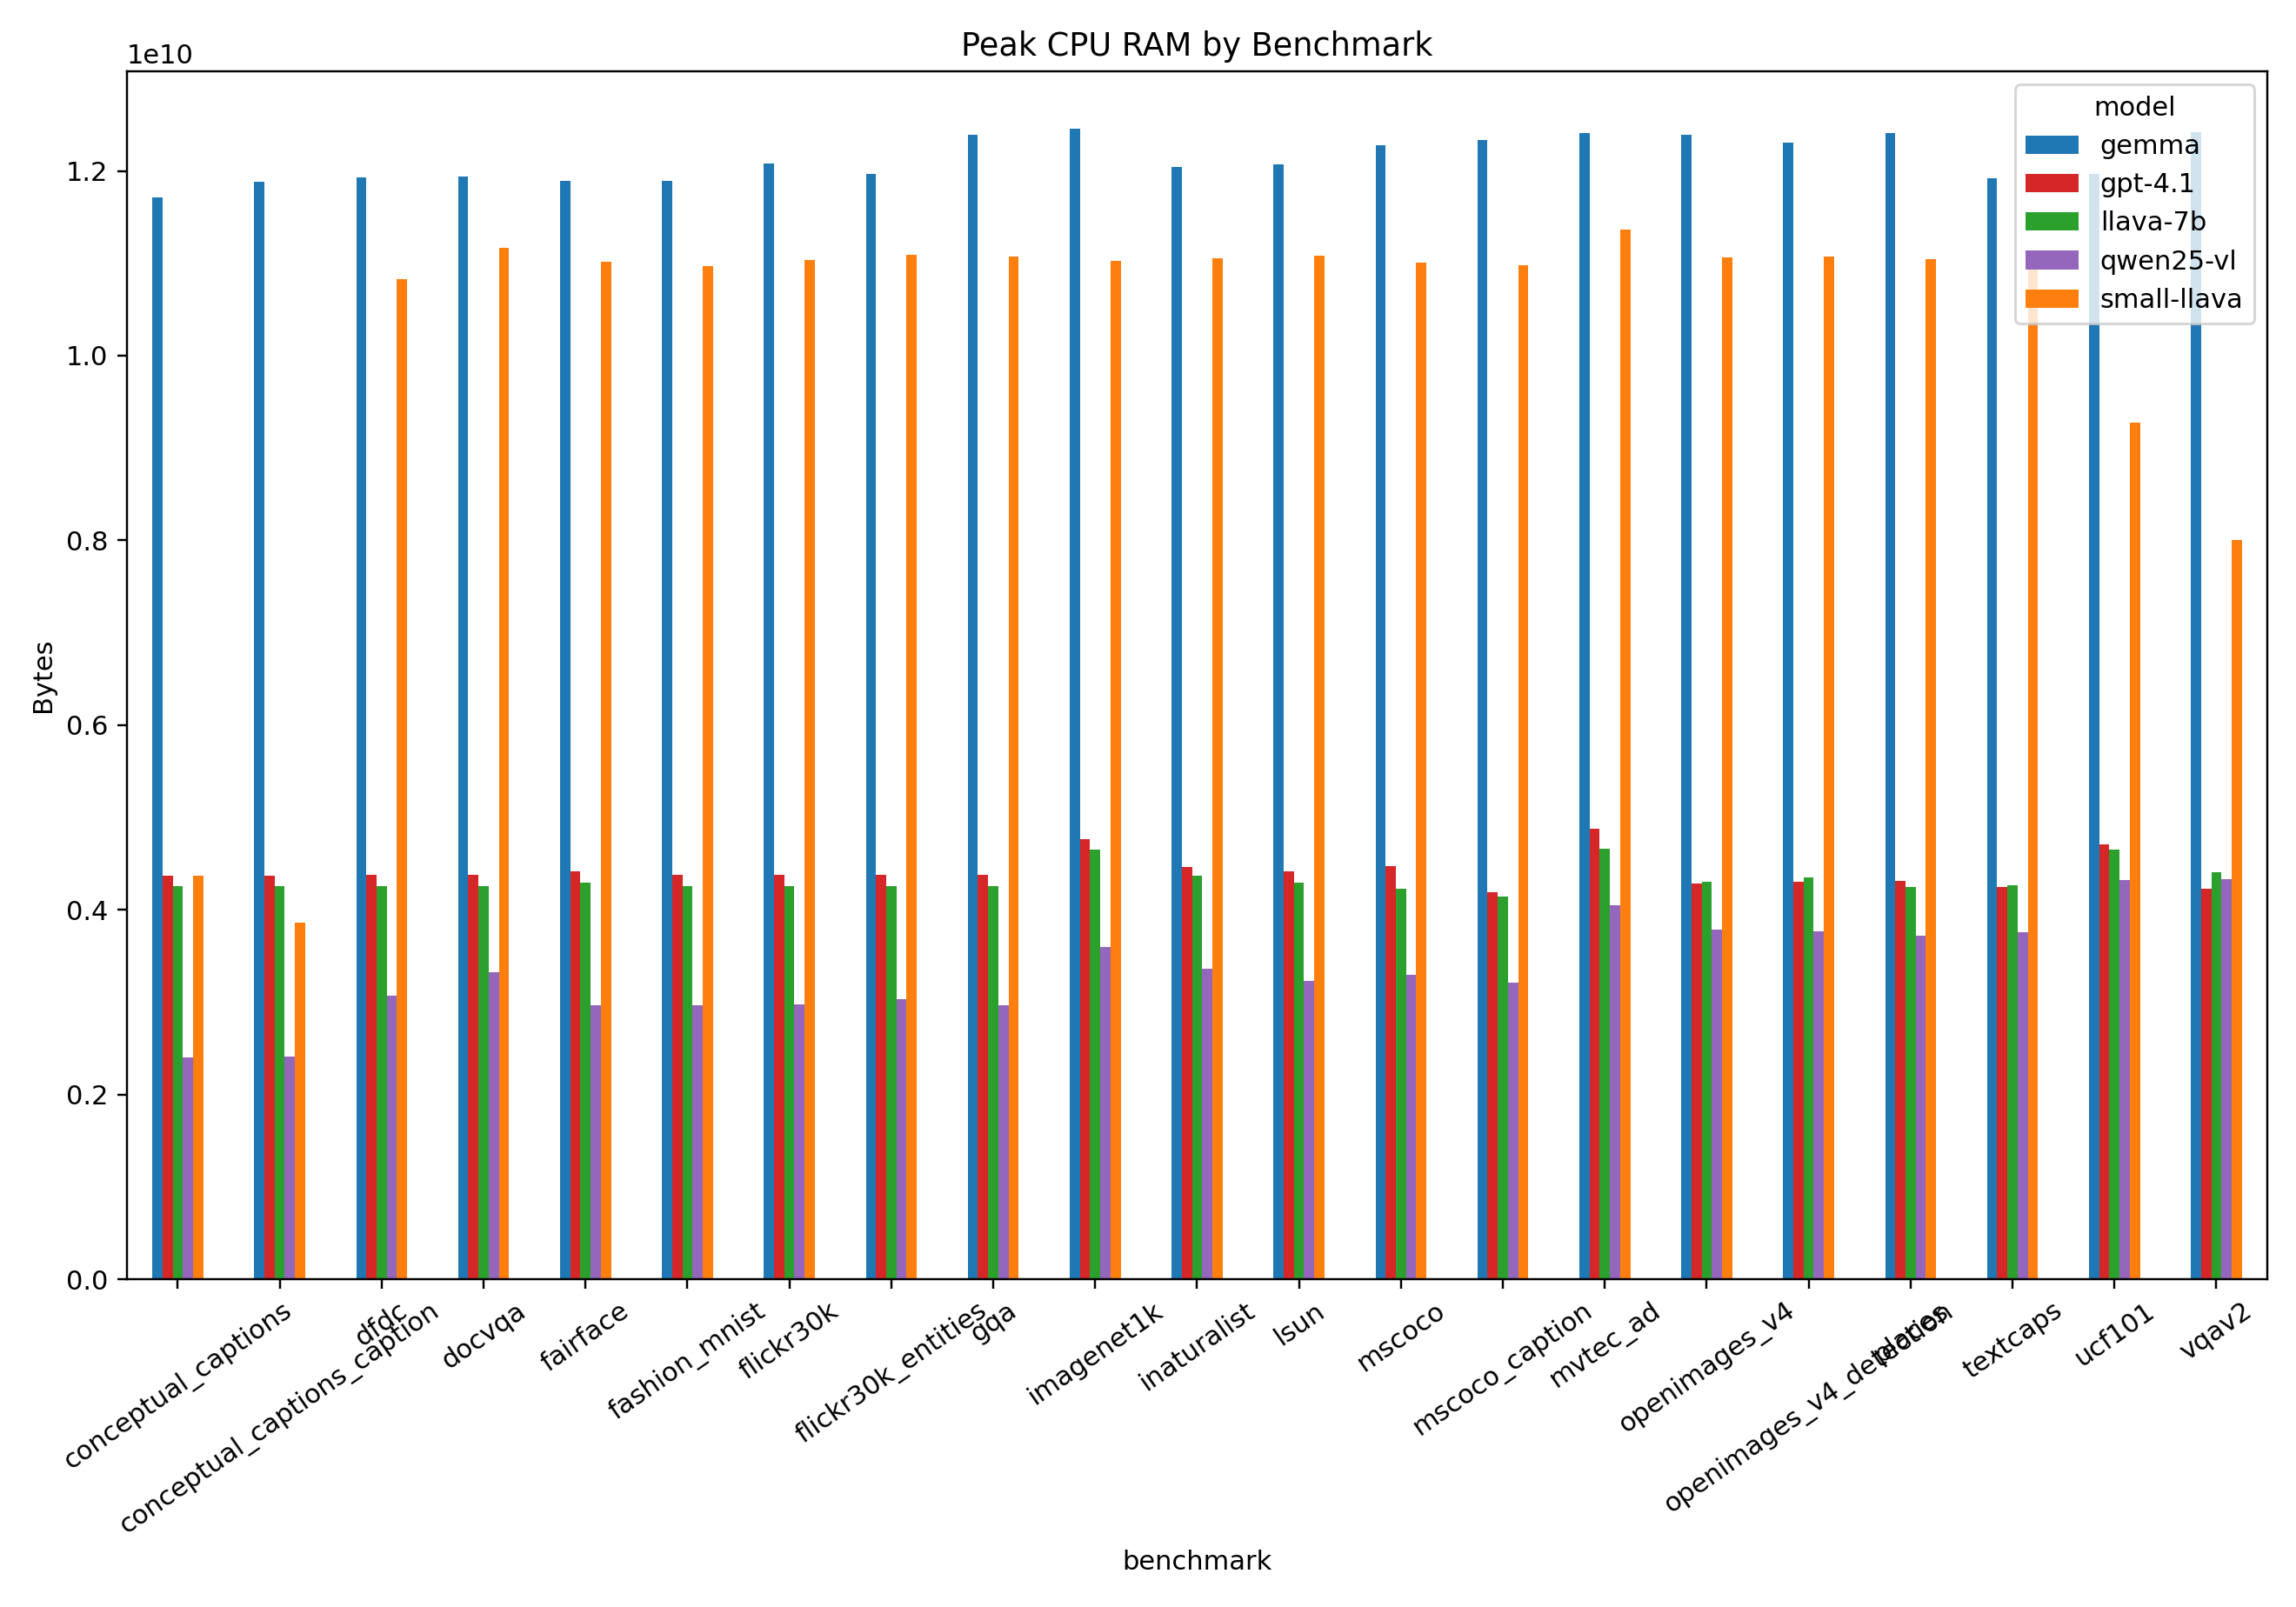
\includegraphics[width=\textwidth]{comparison/output/telemetry_peak_cpu_ram_by_benchmark.png}
\caption{Peak CPU RAM by benchmark.}
\end{figure}

\clearpage
\section{Closing Thought}
What I like about this comparison is that it does not produce a cartoonishly simple winner. \texttt{gpt-4.1} looks best overall, but it wins by being steadier, not by making the other two irrelevant. \texttt{qwen25-vl} is arguably the most impressive pure multimodal competitor here because it wins so often and looks especially natural on captioning. \texttt{llava-7b}, meanwhile, still earns its place by showing how much mileage a comparatively straightforward open multimodal stack can get from a good vision encoder, a projector, and a strong language backbone.

That feels like the human version of the result: three good models, three different design philosophies, and performance differences that mostly make sense once you look at how each system turns images into language.










\section{Comments}

Better not risk speculating as to \textbf{why} some model is better at a kind of task. Compare trade-off

Remember to finish accuracy v. complexity (number of parameters, time). Bubble graph; bubble size could be the number of params

Only fine-tune one or two models for fine-tunning. Something like ``let's see how difficult it is to fine-tune model A yadayada''. Graph of layers finetuned v. accuracy

It's okay to compare medium models (e.g., llava-7b) with large models (e.g., llava-72b)

Write a weekly plan until delivery

Thursday 21 May 10:45

\end{document}
